\documentclass[oneside,a4paper]{extreport}
\usepackage[fontsize=13pt]{fontsize}
% Vietnamee Font 
\usepackage[T5]{fontenc}
\usepackage[utf8]{inputenc}
\DeclareTextSymbolDefault{\DH}{T1}
 % Times New Roman
%\usepackage{newtxtext}
\usepackage{tgtermes}
\usepackage[lite]{mtpro2}
%\usepackage{newtxmath}

% References
\usepackage[
    style=authoryear,
	sorting=nty,
	backend=biber,
    maxcitenames=2,
    mincitenames=1,
    maxbibnames=99,
    uniquelist=false,
]{biblatex}
\usepackage[unicode]{hyperref}
\addbibresource{References/references.bib}
% (name year) -> (name, year)
\DeclareDelimFormat{nameyeardelim}{\addcomma\space}
\DeclareDelimFormat[parencite]{nameyeardelim}{\addcomma\space}

% Defind strings to vietnamese strings
\DefineBibliographyStrings{english}{
    andothers = {\em et al\adddot},
}

\makeatletter
\def\blx@maxline{77}
\makeatother

% Images
\usepackage{graphicx}
\graphicspath{ {Images/} }

% Source Code
\usepackage{listings}
\usepackage{color}
\definecolor{codegreen}{rgb}{0,0.6,0}
\definecolor{codegray}{rgb}{0.5,0.5,0.5}
\definecolor{codepurple}{rgb}{0.58,0,0.82}
\definecolor{backcolour}{rgb}{0.95,0.95,0.92}
\lstdefinestyle{mystyle}{
    backgroundcolor=\color{backcolour},   
    commentstyle=\color{codegreen},
    keywordstyle=\color{magenta},
    numberstyle=\tiny\color{codegray},
    stringstyle=\color{codepurple},
    basicstyle=\footnotesize,
    breakatwhitespace=false,         
    breaklines=true,                 
    captionpos=b,                    
    keepspaces=true,                 
    numbers=left,                    
    numbersep=5pt,                  
    showspaces=false,                
    showstringspaces=false,
    showtabs=false,                  
    tabsize=2
}
\lstset{style=mystyle}

% Algorithm
\usepackage{amsmath}
\usepackage{algorithm}
\usepackage[noend]{algpseudocode}
\makeatletter
\def\BState{\State\hskip-\ALG@thistlm}
\makeatother

% Table
\usepackage{multirow}
\usepackage{array}
\newcolumntype{L}[1]{>{\raggedright\let\newline\\\arraybackslash\hspace{0pt}}m{#1}}
\newcolumntype{C}[1]{>{\centering\let\newline\\\arraybackslash\hspace{0pt}}m{#1}}
\newcolumntype{R}[1]{>{\raggedleft\let\newline\\\arraybackslash\hspace{0pt}}m{#1}}

% Declare alias
\renewcommand{\chaptername}{CHƯƠNG}
\renewcommand{\figurename}{Hình}
\renewcommand{\tablename}{Bảng}
\renewcommand{\contentsname}{MỤC LỤC}
\renewcommand{\listfigurename}{DANH MỤC CÁC HÌNH}
\renewcommand{\listtablename}{DANH MỤC CÁC BẢNG}
\renewcommand{\appendixname}{PHỤ LỤC}

% Line spacing 1.5
\usepackage{setspace}
\setstretch{1.5}
% Indent (Thụt đầu dòng)
\usepackage{indentfirst}

% Marginal
\usepackage[
  top=35mm,
  bottom=30mm,
  left=35mm,
  right=20mm,
  includefoot]{geometry}

% Page numbering
\usepackage{fancyhdr}
\pagestyle{fancy}
\fancyhf{} % clear all header and footer fields
\fancyhead[C]{\thepage} % Centered page numbers of header
\renewcommand{\headrulewidth}{0pt} % no header line
% Redefine plain style (dành cho các trang đầu chương vốn hay bị ép về mặc định)
\fancypagestyle{plain}{
  \fancyhf{}
  \fancyhead[C]{\thepage}
  \renewcommand{\headrulewidth}{0pt}
}

% Cover page (Trang bìa)
\usepackage{tikz}
\usetikzlibrary{calc}
\newcommand\HRule{\rule{\textwidth}{1pt}}

% Define constants (Information Constants)
% ~ is SPACE
\newcommand{\nameStudent}{Nguyễn~Hữu~Tuấn}
\newcommand{\topicName}{Khung~phương~pháp~phân~tích~sắc~thái~cảm~xúc\\của~người~dùng~Việt~Nam~trên~nền~tảng~Youtube\\dựa~trên~kiến~trúc~Transformer}
\newcommand{\mentorName}{Ngô~Tấn~Vũ~Khanh}
\newcommand{\chuyenNganh}{chuyên~ngành~?}
\newcommand{\huongDaoTao}{hướng~đào~tạo~?}
\newcommand{\maSoChuyenNganh}{mã~số~chuyên~ngành~?}

% Fix chapter space before
\usepackage{titlesec}
\titlespacing*{\chapter}{0pt}{-50pt}{20pt}

% Fix toc
\usepackage{tocloft}
\renewcommand{\cftchappresnum}{{\chaptername~} }
\renewcommand{\cftchapaftersnum}{: }
\addtolength{\cftchapnumwidth}{55pt}

% Item-listings
\usepackage{enumitem}

%%%%%%%%%%%%%%%%%%%%%%%%%%%%%%%%%%%%%%%%%%%%%%%%%%%%%%%%%%%%%%%%%%%%%%%%%%%%%%%%%%%%%%%%%%%%
%%% MAIN DOCUMENT!!!                                                                     %%%
%%%%%%%%%%%%%%%%%%%%%%%%%%%%%%%%%%%%%%%%%%%%%%%%%%%%%%%%%%%%%%%%%%%%%%%%%%%%%%%%%%%%%%%%%%%%

\begin{document}

%%%%%%%%%%%%%%%%%%%%%%%%%%%%%%%%%%%%%%%%%%%%%%%%%%%%%%%%%%%%%%%%%%%%%%%%%%%%%%%%%%%%%%%%%%%%
%%% HARD TITLE - MAIN                                                                    %%%
%%%%%%%%%%%%%%%%%%%%%%%%%%%%%%%%%%%%%%%%%%%%%%%%%%%%%%%%%%%%%%%%%%%%%%%%%%%%%%%%%%%%%%%%%%%%

\begin{titlepage}

\begin{center}
    \begin{tikzpicture}[remember picture, overlay]
        % Thick Border
        \draw[line width = 5pt] ($(current page.north west) + (2.0cm,-2.0cm)$) rectangle ($(current page.south east) + (-1.5cm,2.0cm)$);
        % Thin Border
        \draw[line width = 0.5pt] ($(current page.north west) + (2.2cm,-2.2cm)$) rectangle ($(current page.south east) + (-1.7cm,2.2cm)$);
    \end{tikzpicture}

    \vspace{-1.0cm}
    \fontsize{18}{15}\selectfont
    \textbf{BỘ GIÁO DỤC VÀ ĐÀO TẠO}\\
    \textbf{ĐẠI HỌC KINH TẾ THÀNH PHỐ HỒ CHÍ MINH}\\[-1.5ex]
    % small line
    \rule{8.5cm}{0.5pt}\\[3.5cm]

    \fontsize{18}{18}\selectfont
    \textbf{\MakeUppercase{\nameStudent}}\\[2.5cm]

    \fontsize{16}{22}\selectfont
    \textbf{\MakeUppercase{\topicName}}\\[3.5cm]

    \fontsize{18}{18}\selectfont
    \textbf{LUẬN VĂN THẠC SĨ}\\[4cm]

    \vfill
    \fontsize{16}{15}\selectfont
    \textbf{Thành phố Hồ Chí Minh - Năm 2026}

\end{center}

\pagebreak

%%%%%%%%%%%%%%%%%%%%%%%%%%%%%%%%%%%%%%%%%%%%%%%%%%%%%%%%%%%%%%%%%%%%%%%%%%%%%%%%%%%%%%%%%%%%
%%% BREAKING TITLE PAGE                                                                  %%%
%%%%%%%%%%%%%%%%%%%%%%%%%%%%%%%%%%%%%%%%%%%%%%%%%%%%%%%%%%%%%%%%%%%%%%%%%%%%%%%%%%%%%%%%%%%%
\newpage
\cleardoublepage
\thispagestyle{empty}

%%%%%%%%%%%%%%%%%%%%%%%%%%%%%%%%%%%%%%%%%%%%%%%%%%%%%%%%%%%%%%%%%%%%%%%%%%%%%%%%%%%%%%%%%%%%
%%% SOFT TITLE - MAIN                                                                    %%%
%%%%%%%%%%%%%%%%%%%%%%%%%%%%%%%%%%%%%%%%%%%%%%%%%%%%%%%%%%%%%%%%%%%%%%%%%%%%%%%%%%%%%%%%%%%%

\begin{center}
    \begin{tikzpicture}[remember picture, overlay]
        \draw[line width = 5pt] ($(current page.north west) + (2.0cm,-2.0cm)$) rectangle ($(current page.south east) + (-1.5cm,2.0cm)$);
        \draw[line width = 0.5pt] ($(current page.north west) + (2.2cm,-2.2cm)$) rectangle ($(current page.south east) + (-1.7cm,2.2cm)$);
    \end{tikzpicture}

    \vspace{-1.0cm}
    \fontsize{18}{15}\selectfont
    \textbf{BỘ GIÁO DỤC VÀ ĐÀO TẠO}\\
    \textbf{ĐẠI HỌC KINH TẾ THÀNH PHỐ HỒ CHÍ MINH}\\[-1.5ex]
    \rule{8.5cm}{0.7pt}\\[2.5cm]

    \fontsize{18}{15}\selectfont
    \textbf{\MakeUppercase{\nameStudent}}\\[2cm]

    \fontsize{16}{15}\selectfont
    \textbf{\MakeUppercase{\topicName}}\\[1.5cm]
    
    \fontsize{16}{15}\selectfont
    \begin{tabular}{ll}
        Chuyên ngành:  \chuyenNganh\\
        Hướng đào tạo: \huongDaoTao \\
        Mã số: \maSoChuyenNganh
    \end{tabular}\\[2cm]

    \fontsize{18}{18}\selectfont
    \textbf{LUẬN VĂN THẠC SĨ}\\[1.5cm]

    \fontsize{16}{18}\selectfont
    NGƯỜI HƯỚNG DẪN KHOA HỌC:\\
    \MakeUppercase{\mentorName}\\[2cm]

    \vfill
    \fontsize{16}{15}\selectfont
    \textbf{Thành phố Hồ Chí Minh - Năm 2026}

\end{center}

\end{titlepage}


\pagenumbering{roman} % Đánh số i, ii, iii, ...

\clearpage
\phantomsection
\addcontentsline{toc}{chapter}{LỜI CAM ĐOAN}
\chapter*{LỜI CAM ĐOAN}
\label{reassurances}

Luận văn này là kết quả của công trình nghiên cứu khoa học độc lập do chính tôi thực hiện. Toàn bộ liệu và kết quả khảo sát được trình bày đều phản ánh trung thực những gì đã quan sát được, mang tính khách quan và chưa từng xuất hiện trong bất kỳ ấn phẩm khoa học nào trước đây. Mọi lập luận, nhận định và kết luận khoa học được nêu ra xuất phát từ chính quá trình tìm hiểu, phân tích thực tế của tác giả. Riêng phần tài liệu tham khảo được sử dụng, tất cả đều đã được ghi nguồn và trích dẫn đầy đủ, tuân thủ đúng quy định hiện hành.

Toàn bộ quá trình nghiên cứu được hoàn thành dưới sự cố vấn của TS. Ngô Vũ Tấn Khanh. Tác giả cam kết chịu trách nhiệm hoàn toàn trước Hội đồng đánh giá cũng như trước pháp luật về độ xác thực, tính khách quan của nội dung, và về mọi khía cạnh pháp lý có liên quan đến bản quyền.

\hfill
\begin{tabular}{c}
    \textit{Thành phố Hồ Chí Minh, ngày.... tháng.... năm 2026} \\
    \textbf{Tác giả} \\
    \vspace{2.5cm} \\
    \textbf{\nameStudent}
\end{tabular}


\clearpage
\phantomsection
\addcontentsline{toc}{chapter}{LỜI CẢM ƠN}
\chapter*{LỜI CẢM ƠN}
\label{thanks}

Lời đầu tiên, tôi xin bày tỏ lòng biết ơn sâu sắc đến Thầy TS. Ngô Vũ Tấn Khanh, người đã luôn dành sự quan tâm, động viên và hướng dẫn tận tình, chu đáo cho tôi trong suốt thời gian thực hiện và hoàn thành đề án này. Những định hướng khoa học cùng những lời khuyên quý báu của Thầy chính là kim chỉ nam giúp tôi vượt qua nhiều thách thức để hoàn thiện nghiên cứu một cách tốt nhất.

Đồng thời, tôi cũng xin được gửi lời tri ân sâu sắc đến quý thầy, cô tại Trường Đại học Kinh tế Thành phố Hồ Chí Minh (UEH). Với tư cách là những người nhà giáo, quý thầy, cô đã truyền đạt cho tôi những nền tảng kiến thức chuyên môn sâu sắc và vững chắc trong suốt quá trình học tập tại trường. Chính những bài học và sự chỉ dạy tận tâm đó đã góp phần quan trọng giúp tôi định hình, tư duy và hoàn thành kết quả của đề án nghiên cứu này.

Cuối cùng, tôi xin chân thành cảm ơn gia đình, bạn bè và các đồng nghiệp đã luôn bên cạnh động viên, cổ vũ và tạo mọi điều kiện tốt nhất về cả vật chất lẫn tinh thần trong suốt chặng đường học tập và nghiên cứu vừa qua.

Dù đã có nhiều cố gắng, song đề án chắc chắn không tránh khỏi những thiếu sót nhất định. Tôi rất mong nhận được những ý kiến đóng góp, phê bình từ quý thầy, cô và Hội đồng để đề án được hoàn thiện hơn.

Tôi xin chân thành cảm ơn!

\vspace{0.5cm}
\hfill % Đẩy khung ký tên sang góc bên phải
\begin{tabular}{c}
    \textit{Thành phố Hồ Chí Minh, ngày  tháng  năm 2026} \\
    \textbf{Tác giả} \\
    \vspace{2.5cm} \\ % Khoảng trống để ký tên
    \textbf{\nameStudent}
\end{tabular}


\clearpage
\phantomsection
% Mục lục, danh sách hình, danh sách bảng
\addcontentsline{toc}{chapter}{MỤC LỤC}
\tableofcontents
\listoffigures
\listoftables

\clearpage
\phantomsection
\addcontentsline{toc}{chapter}{TÓM TẮT - ABSTRACT}
\chapter*{TÓM TẮT}
\label{tomtat}
Trong bối cảnh YouTube sở hữu lượng người dùng khổng lồ tại Việt Nam, việc phân tích dữ liệu văn bản mang lại tiềm năng to lớn cho các bài toán trong lĩnh vực lắng nghe mạng xã hội. Tuy nhiên, quá trình xử lý ngôn ngữ tiếng Việt trên không gian mạng hiện đang đối mặt với nhiều thách thức do hiện tượng trộn mã (code-switching), sự đa dạng phương ngữ địa phương và biến đổi liên tục của ngôn ngữ mạng. Làm cho các phương pháp máy học truyền thống bộc lộ nhiều hạn chế khi xử lý loại dữ liệu phức tạp này, từ đó tạo động lực cho nghiên cứu nhằm ứng dụng các giải pháp học sâu hiện đại để cải thiện độ chính xác.

Mục tiêu của nghiên cứu này chính là xây dựng một khung phương pháp (framework) chuẩn dựa trên kiến trúc Transformer nhằm phân tích sắc thái cảm xúc của người dùng trên YouTube. Đề tài giải quyết bài toán nhận diện trạng thái tâm lý bằng cách bóc tách 27 trạng thái cảm xúc vi mô có độ hạt mịn cùng một trạng thái trung tính. Khoảng trống nghiên cứu chính là sự thiếu hụt các mô hình có khả năng phân loại cảm xúc chi tiết thay vì chỉ đánh giá phân cực tích cực hay tiêu cực cơ bản.

Nghiên cứu áp dụng phương pháp thực nghiệm định lượng kết hợp các kỹ thuật Xử lý ngôn ngữ tự nhiên tiên tiến. Quy trình thực hiện bao gồm việc thu thập dữ liệu, gán nhãn bán tự động có sự tham gia của Mô hình ngôn ngữ lớn và chuyên gia (LLM-Human-in-the-loop), hiệu chỉnh (fine-tuning) các mô hình ngôn ngữ như mBERT, PhoBERT, mModernBERT kết hợp các kỹ thuật xử lý mất cân bằng lớp.

Kết quả nghiên cứu cho thấy đề tài đã hoàn thiện thành công một chuỗi quy trình chuẩn hóa có khả năng nhận diện chính xác sự phức tạp trong tâm lý người dùng. Quá trình huấn luyện các mô hình đạt được hiệu năng cao, được đánh giá toàn diện qua các độ đo khách quan như F1-macro và Balanced Accuracy để phản ánh trung thực khả năng phân loại trên dữ liệu thực tế.

Kết quả nghiên cứu khẳng định khung phương pháp này có thể áp dụng làm nền tảng kỹ thuật đắc lực cho các hệ thống Lắng nghe mạng xã hội (SociTrong bối cảnh YouTube sở hữu lượng người dùng khổng lồ tại Việt Nam, việc phân tích dữ liệu văn bản mang lại tiềm năng to lớn cho lĩnh vực lắng nghe mạng xã hội. Tuy nhiên, quá trình xử lý ngôn ngữ tiếng Việt trên không gian mạng hiện đang đối mặt với nhiều thách thức do hiện tượng trộn mã (code-switching), sự đa dạng phương ngữ và từ vựng biến đổi liên tục. Các phương pháp máy học truyền thống bộc lộ nhiều hạn chế khi xử lý loại dữ liệu phức tạp này, từ đó tạo động lực cho nghiên cứu nhằm ứng dụng các giải pháp học sâu hiện đại để cải thiện độ chính xác.

\textbf{Từ khóa:} \textit{Phân tích cảm xúc}, \textit{Transformer}, \textit{YouTube}, \textit{Tiếng Việt}, \textit{Social Media Listening}.

\chapter*{ABSTRACT}
\label{abstract}
In the context of YouTube possessing a massive user base in Vietnam, text data analysis offers immense potential for the field of social media listening. However, processing the Vietnamese language in cyberspace currently faces numerous challenges due to code-switching phenomena, dialectal diversity, and constantly evolving vocabulary. Traditional machine learning methods reveal many limitations when handling this complex data type, thereby creating the motivation for this research to apply modern deep learning solutions to improve accuracy.

The objective of this study is to develop a standardized methodological framework based on the Transformer architecture to analyze the emotional nuances of users on YouTube. The research addresses the problem of psychological state recognition by extracting 27 fine-grained micro-emotional states along with a neutral state. The main research gap lies in the lack of models capable of detailed emotion classification, rather than just basic positive or negative sentiment evaluation.

The study applies quantitative experimental methods combined with advanced Natural Language Processing techniques. The implementation process involves data collection, semi-automatic labeling with the participation of Large Language Models and experts (LLM-Human-in-the-loop), and fine-tuning language models such as mBERT, PhoBERT, and mModernBERT, combined with class imbalance processing techniques.

The research results show that the project has successfully developed a standardized pipeline capable of accurately recognizing the complexity of users' psychological states. The training process of the models achieved high performance, comprehensively evaluated through objective metrics such as F1-macro and Balanced Accuracy to truthfully reflect the classification capability on real-world data.

The findings confirm that this methodological framework can be effectively applied as a solid technical foundation for Social Media Listening systems in Vietnam. Businesses and content creators will directly benefit from understanding the community to optimize their business and development strategies. The implication for future research is to continue expanding the dataset and applying this architecture for analysis across various other social media platforms.

\textbf{Keywords:} \textit{Sentiment analysis}, \textit{Transformer}, \textit{YouTube}, \textit{Vietnamese}, \textit{Social Media Listening}.


\clearpage

\pagenumbering{arabic} % Đánh số 1, 2, 3, ...

% Các chương nội dung
\chapter{XÁC ĐỊNH VẤN ĐỀ NGHIÊN CỨU}
\label{Chapter1}

\section{Tính cấp thiết của đề tài}

Ra mắt lần đầu vào năm 2005 và có mặt chính thức tại Việt Nam từ năm 2014, YouTube giờ đây không chỉ là một nền tảng chia sẻ video, mà đã trở thành một kho dữ liệu khổng lồ, mang lại giá trị khai thác cho nhiều lĩnh vực ngành nghề. Theo nghiên cứu của \textcite{choudhury_2019}, Việt Nam hiện nằm trong nhóm 5 thị trường chiến lược hàng đầu, thu hút lượng đầu tư mạnh mẽ bậc nhất từ nền tảng này trên quy mô toàn cầu. Số liệu thống kê từ DataReportal \parencite{kemp_2026} tính đến cuối năm 2025 cũng cho thấy YouTube đang sở hữu tới 62,1 triệu người dùng tại Việt Nam, chiếm 61\% dân số cả nước. Cùng lúc đó, báo cáo của Decision Lab \parencite{decision_lab_2025} ghi nhận tỷ lệ thâm nhập của nền tảng này đạt 87\% trong quý IV/2025 (Hình~\ref{fig:ti_le_tham_nhap}), chỉ đứng sau Facebook, Zalo và bỏ xa TikTok. Những con số này cho thấy hệ sinh thái YouTube đang đường cho các bài toán giám sát thông tin mạng xã hội trực tuyến (Social Media Listening), tức quá trình vận dụng khai thác dữ liệu tiên tiến nhằm theo dõi, chắt lọc thông tin có giá trị từ những cuộc trò chuyện, thảo luận xoay quanh một chủ đề nhất định trên mạng xã hội (chẳng hạn một thương hiệu hay hashtag), qua đó hỗ trợ phát hiện cơ hội kinh doanh, tối ưu hoạt động tiếp thị và nâng cao chất lượng phục vụ người tiêu dùng \parencite{ducange_2019}.

\begin{figure}[htbp]
    \centering
    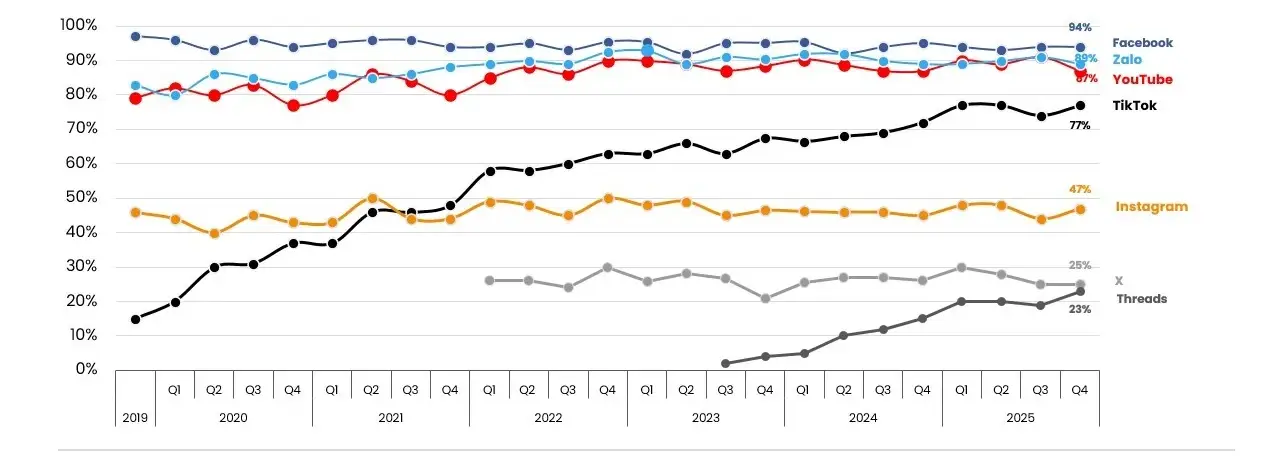
\includegraphics[width=0.8\textwidth]{Images/decision_lab_iv_2025_re.png}
    \caption{Biểu đồ tỷ lệ thâm nhập của các nền tảng mạng xã hội dẫn đầu tại Việt Nam, từ Decision Lab, quý IV 2025}
    \label{fig:ti_le_tham_nhap}
    \vspace{0.1cm}
    {\small Nguồn: \textcite{decision_lab_2025}}
\end{figure}

Những tiến bộ vượt bậc mà \gls{ml} đạt được trong giai đoạn hiện nay đã mở đường cho việc khai thác chuyên sâu các nguồn dữ liệu phi cấu trúc bên cạnh những định dạng có cấu trúc vốn quen thuộc trước đây. Bản thân văn bản là một nguồn tài nguyên thông tin giàu giá trị, lưu giữ các trạng thái nội tâm (private states) của con người như ý kiến, niềm tin, suy nghĩ, tình cảm, cảm xúc, mục tiêu, đánh giá và phán đoán \parencite{wiebe_2005}. Chính vì vậy, việc ứng dụng kỹ thuật \gls{sa} để đo lường mức độ phân cực của ngôn từ là hướng tiếp cận chủ đạo, góp phần nâng cao hiệu quả trích xuất thông tin trên các nền tảng mạng xã hội.

Dù kho dữ liệu công khai trên YouTube có quy mô đồ sộ, đa dạng và mang đặc tính đa miền (multi-domain), các hướng tiếp cận hiện có tại Việt Nam vẫn chưa khai thác hết tiềm năng này và còn tồn tại một số khoảng trống nhất định. Trong khi bài toán nhận diện sắc thái tâm lý trên các ngôn ngữ phổ biến toàn cầu đã đạt được nhiều bước tiến đáng kể \parencite{guo2024mvindemo, zhao2024multi, shen2025zero, zhao2025interpretable, lee2026dimabsa}, thì phần lớn công trình liên quan đến tiếng Việt vẫn bó hẹp trong phạm vi các tập dữ liệu ngách, chỉ giới hạn ở một số miền cụ thể \parencite{minh2024fine, le2025hybrid, nguyen2025like}.

Mặt khác, mặc dù góp mặt trong top 20 ngôn ngữ có cộng đồng người sử dụng đông đảo nhất thế giới \parencite{ethnologue_2026}, tiếng Việt vẫn tiềm ẩn không ít thách thức riêng khi đưa vào xử lý. Trước hết, sự phong phú của các phương ngữ và vốn từ vựng địa phương gây ra không ít trở ngại cho các công cụ xử lý ngôn ngữ tự nhiên (\acrshort{nlp}). Kế đến, sự giao thoa diễn ra trên không gian mạng đã làm cho hiện tượng trộn mã (code-switching) (chẳng hạn: "sản phẩm nhìn rất chill") ngày càng phổ biến và liên tục biến đổi. Thêm vào đó, cách con người diễn đạt cảm xúc luôn thay đổi, cộng với sự xuất hiện của những từ vựng mới, buộc các mô hình ML phải sở hữu khả năng thích nghi cao (adaptability) để không bị suy giảm hiệu năng trước những biến động của ngôn ngữ xã hội.

Đối diện với những thách thức kể trên, các phương pháp cổ điển như hệ thống dựa trên luật (rule-based) hay những kiến trúc mạng học sâu thế hệ trước (\gls{rnn}, \gls{lstm}) dần cho thấy sự hạn chế, bởi chúng thường gặp khó khăn khi phải ghi nhớ thông tin xuyên suốt một chuỗi ngữ cảnh dài và giải mã cấu trúc câu trộn mã phức tạp. Mạng Transformer với cơ chế tự chú ý (Self-Attention) \parencite{vaswani2017attention} giải quyết triệt để rào cản này nhờ khả năng nắm bắt toàn bộ ngữ cảnh văn bản dài mà không phụ thuộc vào khoảng cách, qua đó nâng cao độ chính xác khi xử lý các tác vụ nhận diện thái độ trên dữ liệu đa miền.

Từ những đòi hỏi cấp thiết vừa nêu, câu hỏi được đặt ra là làm thế nào để xây dựng một khung phương pháp (framework) chuẩn hóa, vận dụng kiến trúc Transformer nhằm giải quyết các khó khăn đặc thù của dữ liệu YouTube trong bối cảnh Việt Nam. Đây không chỉ là một bài toán mang giá trị lý luận sâu sắc, mà còn ẩn chứa tiềm năng ứng dụng thực tiễn to lớn. Khung phương pháp được đề xuất sẽ là công cụ hữ-u ích, giúp các nhà sáng tạo nội dung lẫn doanh nghiệp nắm bắt tâm lý khán giả, từ đó có cơ sở vững chắc để hoạch định chiến lược mở rộng nội dung và tối ưu hóa hiệu quả kinh doanh.

\section{Mục tiêu nghiên cứu}

\subsection{Mục tiêu chung}
Xuất phát từ những luận điểm vừa được trình bày, có thể khẳng định rằng xây dựng một khung phương pháp trên nền tảng kiến trúc Transformer, đang trở nên cấp bách, nhằm giải quyết trọn vẹn bài toán nhận diện sắc thái tâm lý của người dùng không chỉ trên YouTube mà còn trên các nền tảng mạng xã hội khác tại Việt Nam. Mục tiêu cốt lõi của khung phương pháp này là tối ưu hóa toàn diện chuỗi công đoạn thiết lập và triển khai vào thực tế, từ việc thu thập dữ liệu trên môi trường internet, tiền xử lý dữ liệu đầu vào, cơ chế gắn nhãn tự động, cho tới khâu mô hình hóa theo hướng bám sát các xu thế công nghệ hiện đại.

Dựa trên thang đo tâm lý mà \textcite{demszky2020goemotions} dựng lên từ cơ sở thực nghiệm của \textcite{cowen2019primacy}, nghiên cứu này hướng đến việc bóc tách và làm rõ tính phức tạp, đa chiều trong trạng thái tâm lý con người thông qua 27 phạm trù cảm xúc vi mô có độ hạt mịn (fine-grained), một bước tiến xa hơn so với hệ thống phân loại sáu lớp cơ bản của \textcite{ekman1992there} hay các cách đánh giá phân cực thô sơ trước đây. Đặc biệt, bằng việc thiết lập bài toán theo hướng phân loại đơn nhãn độc lập, nghiên cứu không hề phủ nhận tính liên tục vốn có của không gian cảm xúc; thay vào đó, trọng tâm được đặt vào việc xây dựng một cơ chế lọc thông tin hiệu quả nhằm xác định chính xác luồng tâm lý chủ đạo (dominant emotion) chi phối mạnh nhất trong mỗi phát ngôn. Nhờ vậy, cách tiếp cận này vừa tận dụng được mật độ thông tin phong phú từ những khám phá tâm lý học hiện đại, vừa đảm bảo tính dứt khoát, rõ ràng cần thiết cho các ứng dụng thực tế ở hạ nguồn trên mạng xã hội nói chung và YouTube nói riêng.

\subsection{Mục tiêu cụ thể}
Để hiện thực hóa định hướng tổng thể đã đề ra, đề án xác định bốn mục tiêu cụ thể, được phân bổ theo trình tự của một quy trình hoàn chỉnh bắt đầu từ khâu thu thập, tổ chức dữ liệu cho đến việc mô hình hóa bằng thuật toán phân lớp với nội dung chi tiết như sau:
\begin{itemize}[label=-]
    \item Xây dựng một kho ngữ liệu quy mô lớn từ việc thu thập và tổng hợp các bình luận (comments) cùng siêu dữ liệu (metadata) liên quan đến video trên YouTube; song song đó, thiết lập quy trình tiền xử lý văn bản để bóc tách và chuẩn hóa các đặc trưng phi cấu trúc, bám sát tiêu chuẩn huấn luyện hiện đại của các mô hình ngôn ngữ lớn trong lĩnh vực \acrshort{nlp}, nhằm khử nhiễu đặc thù của ngôn ngữ mạng trong khi vẫn giữ trọn sắc thái ngữ nghĩa ẩn trong từng ký tự và hành vi tương tác.
    \item Vận dụng lược đồ gồm 27 trạng thái cảm xúc cùng một nhãn trung tính (neutral) do \textcite{demszky2020goemotions} đề xuất, kết hợp cơ chế gán nhãn bán tự động với sự phối hợp giữa chuyên gia và mô hình ngôn ngữ quy mô lớn (LLM-Human-in-the-loop), nhằm xác định chuẩn xác cảm xúc chủ đạo (dominant emotion) hiện diện trong từng văn bản theo cách tối ưu, phù hợp bối cảnh hiện nay.
    \item Thực hiện tinh chỉnh (fine-tuning) các thuật toán học sâu dựa trên bộ khung Transformer đã được tiền huấn luyện chuyên biệt cho tiếng Việt, dù đơn ngữ hay đa ngữ (mBERT, PhoBERT, mModernBERT). Đồng thời áp dụng các kỹ thuật xử lý tình trạng chênh lệch tỷ lệ giữa các nhãn (class imbalance) vốn là đặc trưng của dữ liệu thực tế, trước khi đánh giá chặt chẽ độ ổn định và khả năng khái quát hóa của mô hình thông qua các chỉ số thống kê tiêu chuẩn.
    \item Trên các số liệu thực nghiệm thu thập được, hoàn thiện một quy trình (pipeline) chuẩn hóa có năng lực nhận diện chuẩn xác độ phức tạp trong trạng thái tâm lý người dùng đóng vai trò như một nền tảng kỹ thuật hỗ trợ đắc lực cho giới nghiên cứu thông tin xã hội tại Việt Nam, đồng thời mở đường cho các bài toán ứng dụng ở hạ nguồn (downstream tasks) như nắm bắt thị hiếu, đánh giá sức mạnh thương hiệu, hay kiểm soát và xử lý khủng hoảng truyền thông, được vận hành theo hướng tự động hóa, minh bạch, chuyên sâu và tối ưu chi phí.
\end{itemize}

\subsection{Đối tượng nghiên cứu}
\begin{itemize}[label=-]
    \item \textbf{Về mặt dữ liệu và ngôn ngữ học:} Đối tượng khảo sát tập trung vào các biến động tâm lý, thái độ và sắc thái tình cảm đa chiều của người dùng Việt Nam, được thể hiện thông qua ngữ liệu văn bản phi cấu trúc trên nền tảng YouTube.
    \item \textbf{Về mặt công nghệ và thuật toán:} Trọng tâm nghiên cứu là khai thác các mạng nơ-ron hiện đại vận hành theo cơ chế tự chú ý (Transformer-based models), được huấn luyện riêng cho tiếng Việt lẫn nhiều ngôn ngữ khác; bên cạnh đó, đề án cũng thử nghiệm tích hợp các \gls{llm} để hỗ trợ khâu bóc tách thông tin và rút ngắn thời gian gắn nhãn tự động cho tập dữ liệu.
\end{itemize}

\subsection{Phạm vi nghiên cứu}
\begin{itemize}[label=-]
    \item \textbf{Phạm vi dữ liệu:} Việc thu thập và khai thác ngữ liệu trong đề án được giới hạn trong phạm vi nền tảng YouTube tại thị trường Việt Nam, với dữ liệu đầu vào bao gồm bình luận công khai trích xuất từ video phát lại (\acrshort{vod}) và luồng phát trực tiếp (Livestream), cùng các siêu dữ liệu (metadata) liên quan trực tiếp đến video như tiêu đề, mô tả.
\item \textbf{Phạm vi phân loại cảm xúc:} Thay vì dừng lại ở cách đánh giá cảm tính ba phân lớp ( tiêu cực, tích cực,trung lập) hay hệ thống sáu cảm xúc nền tảng mà \textcite{ekman1992there} khởi xướng, đề án mở rộng phạm vi nhận diện sang không gian cảm xúc hạt mịn (fine-grained emotion categories), cụ thể là lược đồ 27 trạng thái cảm xúc vi mô kết hợp một nhãn trung tính (neutral) do \textcite{demszky2020goemotions} đề xuất, nhằm nắm bắt chuẩn xác các sắc thái biểu đạt phức tạp và đan xen nhau của người dùng trong thực tế.
    \item \textbf{Phạm vi công nghệ áp dụng:} Ở công đoạn gán nhãn có sự phối hợp của chuyên gia (LLM-Human-in-the-loop), đề tài chỉ giới hạn thử nghiệm trên một số \acrshort{llm} tiêu biểu hiện nay như Gemini Flash, Llama 3, Gemma; còn đối với khâu phân loại sắc thái cảm xúc, trọng tâm thực nghiệm là tinh chỉnh (fine-tuning) và đối sánh hiệu năng giữa các kiến trúc Transformer tiền huấn luyện (pre-trained) thuộc họ BERT, bao gồm mBERT, PhoBERT và mModernBERT.
\end{itemize}

\section{Phương pháp nghiên cứu}
Để giải quyết các mục tiêu đã đề ra, đề án triển khai phương thức thực nghiệm định lượng (quantitative empirical research), kết hợp cùng những công nghệ tiên tiến thuộc lĩnh vực Xử lý ngôn ngữ tự nhiên (\acrshort{nlp}) và Học sâu (Deep Learning). Khung phương pháp dựa trên cơ sở tham khảo, kế thừa và tùy biến từ quy trình phân tích cảm xúc của hai công trình \parencite{ding2026scope, hung2026vigoemotions}. Dựa trên nền tảng lý thuyết và thực tiễn vững chắc đó, đề án hệ thống hóa toàn bộ lộ trình thực hiện thành một chuỗi quy trình (pipeline) gồm bốn phân đoạn cốt lõi như sau:

\textbf{Bước 1: Chuẩn bị dữ liệu}
\begin{itemize}[label=-]
    \item Xây dựng danh sách tập hạt giống video dựa trên 15 chủ đề mà YouTube đã phân loại sẵn, không giới hạn công cụ thực hiện.
    \item Vận dụng linh hoạt nhiều phương thức khai thác, trích xuất dữ liệu từ nền tảng này (như Web Scraping, APIs,\dots) nhằm thu thập nội dung liên quan đến người xem (văn bản bình luận, thời điểm đăng tải) cùng hệ thống siêu dữ liệu (metadata) mô tả đặc tính của video như tiêu đề, định danh kênh, thể loại.
    \item Thiết kế và chắt lọc một cơ chế tiền xử lý dữ liệu thô, bám sát những tiêu chuẩn kỹ thuật hiện hành.
\end{itemize}

\textbf{Bước 2: Gán nhãn bán tự động để xây dựng tập ngữ liệu lớn đã được gán nhãn}
\begin{itemize}[label=-]
    \item Lấy mẫu và gán nhãn thủ công, kết hợp cùng tập dữ liệu đối sánh chuẩn (benchmark) ViGoEmotions do \textcite{hung2026vigoemotions} xây dựng, nhằm hình thành tập hạt giống phục vụ cho quá trình gán nhãn tự động.
    \item Lựa chọn một thuật toán đã qua huấn luyện trên kho ngữ liệu văn bản, có độ chính xác đáng tin cậy, để đảm nhiệm việc xử lý phần dữ liệu còn lại chưa được phân loại.
    \item Xây dựng một chu trình phân lớp bán tự động dựa trên mô hình học máy kết hợp cùng tập hạt giống, với mục tiêu mở rộng dần quy mô của tập hạt giống ban đầu và chuyển hóa nó thành một dữ liệu đầu vào có độ chính xác cao.
\end{itemize}

\textbf{Bước 3: Hiệu chỉnh mô hình}
\begin{itemize}[label=-]
    \item Áp dụng các kỹ thuật khử mất cân đối giữa các nhãn khi hiệu chỉnh những mạng học sâu được lựa chọn cho khâu mô hình hóa.
    \item Vận dụng cơ chế học chuyển giao (Transfer Learning) để mô hình thích nghi với bộ dữ liệu đã thu thập được ở các khâu trước, qua đó kế thừa năng lực phân tích vượt trội của những mô hình ngôn ngữ quy mô lớn (vốn đã được huấn luyện trên kho ngữ liệu phong phú), giúp đẩy nhanh khả năng thích ứng với các biến thể phức tạp của văn phong trên internet.
\end{itemize}

\textbf{Bước 4: Đánh giá và so sánh kết quả}
\begin{itemize}[label=-]
    \item Bởi mục tiêu then chốt là xây dựng một phương pháp luận tương thích trọn vẹn với nền tảng Transformer, việc kiểm định hiệu quả học máy sau khi mô hình hóa là bước bắt buộc, nhằm đưa ra những nhận định trung thực và khách quan
    \item Bởi bản chất dữ liệu vốn đã mất cân bằng một cách tự nhiên, việc đánh giá cần dựa trên các độ đo khách quan như F1-macro và Balanced Accuracy để bổ trợ cho độ đo độ chính xác tổng thể (Overall Accuracy).
\end{itemize}

\section{Bố cục của đề án}

Bám sát khung phương pháp luận đã đề xuất cùng những mục tiêu đã xác lập, nội dung của công trình được tổ chức thành 5 chương cốt lõi, trình bày theo thứ tự như sau:

\begin{itemize}
    \item \textbf{Chương 1: Xác định vấn đề nghiên cứu} - Trình bày bối cảnh và tính cấp thiết của đề tài, làm rõ mục đích, mục tiêu, đối tượng, phạm vi cũng như phương pháp nghiên cứu, đồng thời giới thiệu khái quát bố cục của đồ án.
    \item \textbf{Chương 2: Lược khảo cơ sở lý thuyết và các nghiên cứu trước} - Hệ thống hóa các khái niệm nền tảng phục vụ việc xây dựng khung phương pháp, bao gồm khung phương pháp luận, bài toán phân tích sắc thái cảm xúc, kiến trúc Transformer, cùng các công trình liên quan đã công bố trong và ngoài nước, qua đó định hình bức tranh tổng thể của bài toán.
    \item \textbf{Chương 3: Phương pháp nghiên cứu} - Trình bày cụ thể quá trình xây dựng khung phương pháp, bao quát từ thu thập dữ liệu, tiền xử lý, đến khâu mô hình hóa và đánh giá kết quả.
    \item \textbf{Chương 4: Kết quả nghiên cứu và thảo luận} - Mô tả môi trường thực nghiệm cùng các tham số cấu hình, triển khai đối sánh quá trình huấn luyện giữa các mô hình và phân tích định lượng dựa trên các độ đo tiêu chuẩn (Overall Accuracy, Balanced Accuracy, F1-macro) trên tập kiểm định, từ đó đưa ra những đánh giá khách quan về hiệu năng thực tế của toàn bộ khung phương pháp.
    \item \textbf{Chương 5: Kết luận và hàm ý} - Đúc kết những đóng góp chính của nghiên cứu và đề xuất các hướng phát triển tiếp theo.
\end{itemize}

\section{Khoảng trống và động lực nghiên cứu}

Qua những luận điểm đã trình bày, có thể nhận thấy lĩnh vực phân tích sắc thái cảm xúc (\acrshort{sa}) tuy đang nhận được sự quan tâm sâu rộng từ giới khoa học, nhưng khi đặt vào bối cảnh thực tế phức tạp của nền tảng YouTube tại Việt Nam, chủ đề này vẫn còn tồn đọng những khoảng trống chưa được giải quyết trọn vẹn, cả về mặt lý luận lẫn ứng dụng.

Thứ nhất, đa số các công trình trước đây về nghiên cứu cảm xúc trong văn bản tiếng Việt vẫn chủ yếu dừng ở mức phân cực thô sơ (ba mức: tích cực, tiêu cực, trung tính) và sử dụng các thuật toán học máy truyền thống hay mạng nơ-ron thế hệ cũ (như \acrshort{rnn}, \acrshort{lstm}) để mô hình hóa. Cho đến nay, vẫn chưa xuất hiện công trình nào xây dựng và kiểm chứng một khung phương pháp (framework) chuẩn có khả năng kết nối thang đo 27 trạng thái cảm xúc vi mô cùng một nhãn trung tính với các kiến trúc Transformer tiên tiến như PhoBERT hay mModernBERT, song song với cơ chế gán nhãn bán tự động (LLM-Human-in-the-loop), nhằm khai thác đồng thời hai lợi thế: khả năng nhận diện cảm xúc hạt mịn (fine-grained) và năng lực bóc tách ngữ cảnh vượt trội của các mạng học sâu hiện đại được huấn luyện trên khối lượng ngữ liệu khổng lồ.

Thứ hai, một rào cản lớn khác trong bài toán lắng nghe mạng xã hội nằm ở tình trạng sai lệch và tính đa nghĩa phức tạp của văn phong đời thực. Phần lớn công trình trước đây thường dựa vào những kho ngữ liệu đã được làm sạch triệt để, chấp nhận đánh đổi giữa tính toàn vẹn của cảm xúc trong ngữ liệu với hiệu năng mô hình, hoặc chỉ giới hạn trong các miền cụ thể như đánh giá nhà hàng, khách sạn, điện thoại. Trong khi đó, bình luận trên YouTube trong thực tế lại mang đặc tính đa miền (multi-domain), chứa nhiều hiện tượng trộn mã (code-switching), từ lóng, cùng tình trạng mất cân bằng phân lớp nghiêm trọng. Do đó, việc xây dựng một cơ chế tiền xử lý bám sát thực tiễn bao gồm chuẩn hóa ngôn ngữ mạng, trích xuất đặc trưng tương thích với các kiến trúc học sâu quy mô lớn, và áp dụng hợp lý các kỹ thuật khử mất cân bằng dữ liệu đang trở thành một yêu cầu cấp thiết, nhưng vẫn chưa nhận được sự đầu tư tương xứng trong môi trường ứng dụng tại Việt Nam.

Thứ ba, phần đông các học giả, nhà nghiên cứu và kỹ sư dữ liệu hiện nay có xu hướng đánh giá chất lượng mạng nơ-ron trong việc phân tích cảm xúc dựa vào độ chính xác tổng thể (Overall Accuracy), trong khi bỏ ngỏ việc đo lường toàn cảnh quá trình huấn luyện. Hệ quả là khâu từ chuẩn bị dữ liệu đến biểu diễn kết quả thiếu đi tính bao quát cần thiết, đặc biệt khi triển khai trong môi trường thực tế, nơi độ chuẩn xác của dữ liệu đầu ra luôn phụ thuộc trực tiếp vào sự liền mạch, thông suốt giữa các mắt xích trong toàn bộ quy trình.

Trong ngách phân tích văn bản hiện đại, kiến trúc Transformer \parencite{vaswani2017attention} và các mô hình \acrshort{llm} đều đã khẳng định vai trò trung tâm — vế đầu nhờ khả năng nắm bắt ngữ cảnh dài qua cơ chế tự chú ý, vế sau nhờ năng lực suy luận, tự động hóa các tác vụ như gán nhãn. Tuy chưa có nhiều công trình chính thức tại Việt Nam ứng dụng trọn vẹn sự kết hợp giữa hệ thống 27+1 nhãn cảm xúc vi mô với nền tảng kiến trúc Transformer cho dữ liệu YouTube, nhưng ở quy mô các hệ ngôn ngữ lớn trên thế giới, sự tích hợp này đã chứng minh hiệu quả tích cực trong việc phân lớp và nắm bắt tâm lý phức tạp của người dùng. Vì vậy, đề án này kế thừa những thành tựu tiên tiến từ cộng đồng quốc tế để đề xuất một quy trình (pipeline) chuẩn hóa, tận dụng đồng thời năng lực học chuyển giao của các mô hình họ BERT và hệ thống phân loại hạt mịn, từ đó nâng cao hiệu suất nhận diện cảm xúc trong điều kiện dữ liệu thực tế vốn nhiều nhiễu và biến động.

Trên cơ sở những hạn chế còn tồn đọng vừa được phân tích, đề án "Khung phương pháp phân tích sắc thái cảm xúc của người dùng Việt Nam trên nền tảng YouTube dựa trên kiến trúc Transformer" không chỉ mang ý nghĩa như một đóng góp lý luận nhờ quy trình kết hợp mang tính đột phá, mà còn mở ra triển vọng lớn cho việc nâng cấp toàn diện các công cụ giám sát mạng xã hội (Social Media Listening), phục vụ trực tiếp cho các nhãn hàng và đội ngũ sản xuất nội dung số tại Việt Nam trong bối cảnh hiện nay.

\chapter{LƯỢC KHẢO CƠ SỞ LÝ THUYẾT VÀ NGHIÊN CỨU TRƯỚC}
\label{Chapter2}

\section{Tổng quan về bài toán phân tích sắc thái cảm xúc}

\subsection{Cảm xúc và sắc thái tâm trạng qua lăng kính tâm lý học}
Trong cuộc sống hàng ngày, khái niệm cảm xúc (emotion) và sắc thái tâm trạng (sentiment) thường được dùng để thay thế lẫn nhau. Tuy nhiên, trong lĩnh vực tâm lý học, chúng được coi là hai khái niệm khác biệt. Trong mô hình tâm lý học nổi tiếng mà \textcite{watson1985toward} xây dựng, đã chỉ ra cảm xúc mang cấu trúc hai chiều. Dựa trên đó, cảm xúc được định nghĩa là một trạng thái tâm lý cốt lõi phát sinh tức thời, bao gồm ba thành phần cấu trúc: trải nghiệm chủ quan, phản ứng sinh lý và phản ứng hành vi. Nhà tâm lý học \textcite{ekman1992there} đã phân loại cảm xúc thành sáu nhóm cơ bản (hạnh phúc, buồn bã, tức giận, sợ hãi, ngạc nhiên, ghê tởm), và sau này được mở rộng với các trạng thái thứ cấp như hào hứng, xấu hổ, khinh thường và thẹn thùng.

Ngược lại, sắc thái tâm trạng (sentiment) là một thái độ tinh thần mang tính tổ chức cao, được bồi đắp và hình thành dựa trên nền tảng của các cảm xúc sơ cấp. Định nghĩa này nhấn mạnh rằng "sentiment" được sử dụng để truyền tải những suy nghĩ của một cá nhân bắt nguồn từ chính cảm xúc của họ. Không giống như cảm xúc, "sentiment" tiến xa hơn một bước và không bị giới hạn trong các chiều không gian tâm lý thuần túy \parencite{yue2019survey}. Theo \textcite{mcdougall2015introduction}, sắc thái tâm trạng đóng vai trò như cầu nối giữa cảm xúc cốt lõi và chuỗi hành động có chủ đích. Nói cách khác, các loại cảm xúc đa dạng đóng vai trò như những nhân tố cấu thành nên sắc thái tâm trạng tổng thể của một cá nhân đối với một sự vật, sự việc.

\subsection{Cơ sở thần kinh học của sự biểu hiện và hiện tượng suy hao cảm xúc trong văn bản}
Dựa trên cơ sở lý thuyết của các nhà tâm lý học, các nhà khoa học thần kinh đã tiến sâu vào giải mã cơ chế sinh học của quá trình hình thành và truyền đạt cảm xúc.

Khi con người tiếp nhận một kích thích từ môi trường, tín hiệu ngay lập tức được truyền qua đồi thị (Thalamus) đến hạch hạnh nhân (Amygdala) - trung tâm xử lý cảm xúc cốt lõi, đồng thời truyền đến vỏ não trước trán (Prefrontal Cortex) để phân tích nhận thức \parencite{ledoux2013emotion}. Sau đó, hệ thần kinh tự chủ (Autonomic Nervous System) phản ứng bằng cách thay đổi nhịp tim, nhịp thở, tạo ra các "cảm giác" về mặt thể chất. Kết quả của quá trình này là các hành vi biểu hiện cảm xúc ra bên ngoài thông qua nét mặt, cử chỉ hoặc ngôn ngữ.

Tuy nhiên, khi cảm xúc phức tạp này được mã hóa xuống cấp độ ngôn ngữ dưới dạng văn bản thuần túy, một lượng lớn thông tin bị triệt tiêu. Theo nguyên tắc giao tiếp nổi tiếng của Albert Mehrabian, từ ngữ (ngôn từ) chỉ chiếm khoảng 7\% khả năng truyền tải ý nghĩa cảm xúc, phần còn lại phụ thuộc vào ngữ điệu giọng nói (38\%) và ngôn ngữ cơ thể (55\%) \parencite{mehrabian1971silent}. Do đó, một văn bản chữ viết đã đánh mất đến 93\% các manh mối cảm xúc phi ngôn ngữ.

Đối với người tiếp nhận, quá trình giải mã cảm xúc cũng sẽ đi qua một chu trình thần kinh phức tạp. Tín hiệu đầu vào (đọc văn bản, nghe âm thanh, nhìn nét mặt) được xử lý thông qua hệ thống nơ-ron gương (Mirror Neuron System) trong não bộ. Các nơ-ron này kích hoạt sự "mô phỏng" tự động, ra lệnh cho cơ thể tái hiện lại trạng thái cảm giác của người phát tín hiệu. Tín hiệu mô phỏng này sau đó được chuyển đến thùy đảo (Insula) và hạch hạnh nhân để não bộ có thể thực sự "cảm nhận", từ đó phân tích và ra quyết định phân loại sắc thái tâm trạng đó là tích cực, tiêu cực hay trung tính \parencite{iacoboni2009imitation}.

\subsection{Bài toán phân tích sắc thái cảm xúc và các cấp độ phân tích}

\textbf{Phân tích sắc thái cảm xúc (Sentiment Analysis - SA)}, hay còn được gọi là khai thác ý kiến (Opinion mining), là lĩnh vực nghiên cứu chuyên sâu về các quan điểm, thái độ và cảm xúc của con người được diễn đạt thông qua ngôn ngữ văn bản \parencite{liu2010sentiment}. Về mặt kỹ thuật, tác vụ này không chỉ dừng lại ở việc nhận diện từ vựng mang tính cảm xúc, mà là một quy trình trích xuất và phân loại các thông tin mang tính chủ quan nhằm xác định chính xác thái độ của người viết hướng tới một thực thể cụ thể \parencite{liu2010sentiment}.

Trong bài toán phân tích sắc thái cảm xúc, thuật ngữ \textit{đối tượng} ($o$) thường được dùng để chỉ thực thể mục tiêu mà người viết hướng tới, chẳng hạn như sản phẩm, dịch vụ, cá nhân hoặc tổ chức. Về mặt cấu trúc, một đối tượng $o$ có thể được phân tách thành một hệ thống phân cấp bao gồm các thành phần ($T$) và các thuộc tính ($A$). Chẳng hạn, nếu xét đối tượng $o$ là một "Video", các thành phần $T$ có thể bao gồm "nội dung", "âm thanh", "diễn viên"; các thuộc tính $A$ tương ứng có thể là "độ chân thực" hay "kỹ năng diễn xuất". Và trong đó, bản thân các thành phần này cũng có thể tiếp tục chia nhỏ thành các thành phần con $T_1$ như "phân cảnh", "thông điệp truyền tải", "lời thoại",... và các thuộc tính con $A_1$ như "độ hấp dẫn", "độ sâu sắc", "tính logic",...

Dựa trên định nghĩa này, đối tượng $o$ có thể được biểu diễn dưới dạng một cấu trúc cây phân cấp $o: (T, A)$, trong đó gốc là chính đối tượng $o$, các nút trong là các thành phần và các lá đại diện cho các thuộc tính chi tiết. Mặc dù cảm xúc có thể được biểu đạt tại bất kỳ nút nào trên cây, nhưng việc khai thác trực tiếp trên cấu trúc này thường gặp khó khăn do độ phức tạp về mặt tính toán và xử lý ngôn ngữ tự nhiên.

Do vậy, để tối ưu hóa quá trình khai thác, cấu trúc cây thường được đơn giản hóa bằng phương pháp "làm phẳng" (flattening). Khi đó, tất cả các thành phần và thuộc tính được gọi chung bằng thuật ngữ \textbf{khía cạnh} (aspect) hoặc \textbf{đặc tính} (feature), ký hiệu là $f$. Dựa trên nền tảng này, một ý kiến (opinion) sẽ được mô hình hóa chính thức dưới dạng một \textit{bộ năm thành phần (quintuple)} $(o, f, so, h, t)$, trong đó:   
\begin{itemize}
\item $o$: Đối tượng mục tiêu biểu đạt cảm xúc hay ý kiến trong văn bản.
\item $f$: Khía cạnh của đối tượng được đánh giá.
\item $so$: Hướng cảm xúc (sentiment orientation), thường mang giá trị tích cực, tiêu cực hoặc trung tính.
\item $h$: Chủ thể (holder) diễn đạt cảm xúc.
\item $t$: Thời điểm cảm xúc được biểu đạt.
\end{itemize} 
Và đối với một văn bản $d = \langle s_1, s_2, \dots, s_m \rangle$, trong đó $s_i$ là các câu cấu thành, mục tiêu của việc phân tích cảm xúc được phân định rõ ràng qua ba cấp độ nghiên cứu chính:
\begin{itemize}
    \item \textbf{Cấp độ văn bản (Document-level):} Xác định hướng cảm xúc tổng thể của toàn bộ văn bản $d$ đối với đối tượng $o$, thường được biểu diễn bằng cặp $(o, so)$.
    \item \textbf{Cấp độ câu (Sentence-level):} Xác định cảm xúc của từng câu $s_i$ đối với đối tượng $o$. Cấp độ này thường đi kèm với nhiệm vụ phân loại tính chủ quan (subjectivity classification) để phân tách câu chứa ý kiến và câu nêu sự thật.
    \item \textbf{Cấp độ khía cạnh (Aspect-level):} Xác định hướng cảm xúc đối với từng khía cạnh cụ thể $f_j$ của đối tượng $o$ được đề cập trong câu $s_i$, biểu diễn bằng bộ $(s_i, f_j, so)$. Đây là cấp độ chi tiết nhất, cho phép xử lý các văn bản chứa nhiều ý kiến phức tạp và trái ngược nhau.
\end{itemize}

\subsection{Phân tích sắc thái cảm xúc trên nền tảng học máy}

Như đã lập luận ở phần cơ sở thần kinh học, quá trình chuyển hóa cảm xúc thành văn bản thuần túy gây ra hiện tượng suy hao thông tin nghiêm trọng (lên đến 93\% các manh mối phi ngôn ngữ). Khi con người đọc văn bản, hệ thống nơ-ron gương (Mirror Neuron System) trong não bộ phải hoạt động liên tục để "mô phỏng" và bù đắp lượng thông tin khuyết thiếu này. Tuy nhiên, đối với máy tính, các phương pháp phân tích văn bản truyền thống dựa trên luật (rule-based) hoặc từ điển (lexicon) hoàn toàn bất lực trong việc khôi phục các tín hiệu cảm xúc ẩn, bởi chúng chỉ phân tích bề mặt từ vựng mà bỏ qua ngữ cảnh và cấu trúc ngữ nghĩa sâu xa \parencite{liu2012sentiment}.

Để giải quyết thách thức này, các phương pháp tiếp cận dựa trên Học máy (Machine Learning) và Học sâu (Deep Learning) ra đời, đóng vai trò như một "hệ thống nơ-ron gương kỹ thuật số". Thay vì dựa vào các quy tắc cứng nhắc, các thuật toán học máy có khả năng tự động trích xuất các biểu diễn đặc trưng phi tuyến tính (non-linear representations) từ các tập dữ liệu lớn. Thông qua việc phân tích tần suất xuất hiện, vị trí, và mối liên kết ngữ cảnh giữa các từ, hệ thống có thể học cách suy luận và dự đoán sắc thái tâm trạng một cách tự động và chính xác.

Sự phát triển của phân tích sắc thái cảm xúc trên nền tảng học máy trải qua các giai đoạn chính:
\begin{itemize}
    \item \textbf{Học máy truyền thống (Traditional Machine Learning):} Các thuật toán như Support Vector Machine (SVM), Naive Bayes, hay Logistic Regression sử dụng các kỹ thuật trích xuất đặc trưng thủ công như Bag-of-Words (BoW) hoặc TF-IDF. Mặc dù mang lại hiệu quả cao hơn phương pháp từ điển, nhóm này vẫn gặp hạn chế lớn trong việc hiểu chuỗi ngữ cảnh dài và thứ tự từ vựng.
    \item \textbf{Học sâu (Deep Learning):} Sự ra đời của các Mạng nơ-ron nhân tạo (Artificial Neural Networks) như RNN, CNN, LSTM và đặc biệt là kiến trúc Transformer đã tạo ra bước đột phá. Các mô hình này có khả năng nhúng từ vựng vào một không gian véc-tơ đa chiều (Word Embeddings), giúp biểu diễn trọn vẹn mối quan hệ ngữ nghĩa tinh vi và tự động phân tách đối tượng $o$ cùng khía cạnh $f$ trong bộ năm thành phần $(o, f, so, h, t)$.
\end{itemize}

Về mặt định nghĩa toán học, quá trình phân tích sắc thái cảm xúc bằng học máy là việc xấp xỉ một hàm mục tiêu để ánh xạ từ không gian văn bản đầu vào sang không gian nhãn cảm xúc. Gọi $\mathcal{D} = \{d_1, d_2, \dots, d_n\}$ là tập hợp các văn bản (hoặc câu, bình luận) cần phân tích. Gọi $\mathcal{E}$ là không gian nhãn cảm xúc được định nghĩa trước (ví dụ: $\mathcal{E} = \{Tích\ cực, Tiêu\ cực, Trung\ tính\}$ đối với phân loại 3 cực).

\subsection{Tổng quan về các thách thức phân tích sắc thái cảm xúc trên nền tảng YouTube}

\section{Tổng quan về phương pháp luận - Methodological Framework}
Hiện nay, cộng đồng học thuật vẫn chưa có một định nghĩa chính thức về \textbf{khung phương pháp luận (methodological framework)}. Tuy nhiên, có một sự đồng thuận ngầm rằng đây là một công cụ giúp dẫn dắt người thực hiện đi qua một chuỗi các bước có trình tự để hoàn thành một quy trình cụ thể. Trong đó, \textbf{phương pháp luận} được hiểu là tập hợp các phương pháp trong một lĩnh vực chuyên biệt, còn \textbf{khung} đóng vai trò là cấu trúc của các quy tắc hoặc ý tưởng nền tảng. Việc áp dụng khung phương pháp luận không chỉ giúp cải thiện tính nhất quán, tính chặt chẽ mà còn chuẩn hóa các cách tiếp cận, từ đó tối đa hóa độ tin cậy của các kết quả nghiên cứu \parencite{mcmeekin2020methodological}.

Dựa trên các tiền đề đó, một khung phương pháp luận chất lượng cần đáp ứng các tiêu chí cốt lõi sau.

    \begin{itemize}
        \item \textbf{Tính hệ thống (Systematicity)}: Các bước phải được sắp xếp theo trình tự logic, có sự liên kết chặt chẽ và nhất quán xuyên suốt quy trình.
        \item \textbf{Tính toàn diện (Comprehensiveness)}: Bao quát đầy đủ các giai đoạn cần thiết, từ khâu xác định bằng chứng đến khâu thực thi và đánh giá.
        \item \textbf{Tính linh hoạt (Flexibility)}: Có khả năng điều chỉnh và thích nghi với các bối cảnh nghiên cứu khác nhau mà không phá vỡ cấu trúc cốt lõi.
        \item \textbf{Tính khả thi và Thực chứng (Feasibility \& Evidence-based)}: Khung phải được xây dựng dựa trên dữ liệu thực tế, kinh nghiệm chuyên gia và có khả năng ứng dụng thực tiễn cao thông qua việc thử nghiệm (pilot).
    \end{itemize}

    Với phạm vi đề tài, trong các nghiên cứu gần đây về xây dựng khung phương pháp cho bài toán phân tích cảm xúc (Sentiment Analysis), dù thực hiện trên dữ liệu tiếng Việt hay các ngôn ngữ khác, quy trình thực hiện đa phần đều tuân thủ các giai đoạn chuẩn hóa bao gồm: thu thập dữ liệu, tiền xử lý, tách từ (tokenization) và vector hóa, huấn luyện mô hình, và cuối cùng là đánh giá, biểu diễn kết quả (\cite{el2025transformer}, \cite{singh2021youtube}). Quy trình hệ thống này cũng tương đồng với khung phương pháp luận do Uma Maheswari cùng các cộng sự đề xuất (Hình \ref{fig:sa_framework}).

    \begin{figure}[H]
        \centering
        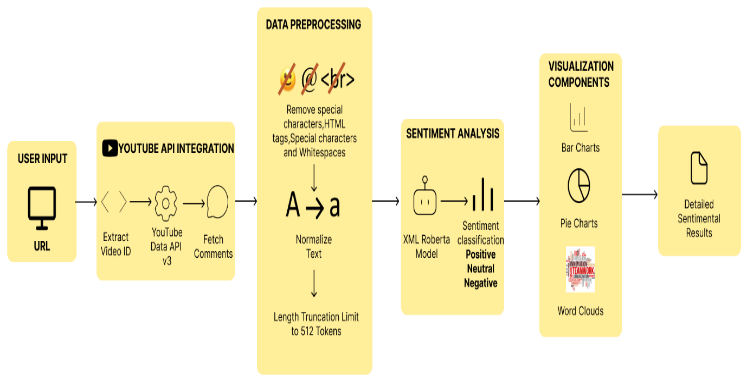
\includegraphics[width=0.8\textwidth]{Images/framework_sample.png}
        \caption{Khung phương pháp luận chung cho bài toán phân tích sắc thái cảm xúc được Uma Maheswari cùng các cộng sự đề xuất \cite{Maheswari2024Sentiment}.}
        \label{fig:sa_framework}
    \end{figure}

    Ngoài ra, khi khảo sát các công trình nghiên cứu chuyên biệt về văn bản tiếng Việt cho thấy, trọng tâm hiện nay chủ yếu tập trung vào việc cải tiến cấu trúc các mô hình học máy nhằm tối ưu hóa độ chính xác (\cite{minh2024fine}, \cite{nguyen2025like}, \cite{quoc2023vietnamese}). Tuy nhiên, xu hướng này dẫn đến việc ưu tiên quá mức các chỉ số định lượng (như Accuracy, F1-score) trên các bộ dữ liệu mẫu (benchmark datasets) mà chưa chú trọng đúng mức đến việc xây dựng một quy trình xử lý chuẩn hóa có tính thích ứng cao. Hệ quả là các mô hình thường đạt hiệu suất tối ưu trong môi trường thực nghiệm nhưng lại bộc lộ hạn chế về tính linh hoạt khi triển khai trên dữ liệu thực tế — nơi ngôn ngữ biến đổi liên tục và có độ nhiễu cao như các bình luận trên nền tảng YouTube.

\section{Tổng quan về các mô hình dựa trên Transformer}

\textbf{Kiến trúc Transformer}, được giới thiệu bởi Vaswani và các cộng sự \cite{vaswani2017attention}, đã tạo nên một bước ngoặt quan trọng trong lĩnh vực xử lý ngôn ngữ tự nhiên (NLP). Mà trọng tâm của kiến trúc này là cơ chế tự chú ý (Self-Attention) (Hình \ref{fig:attetion}), cho phép mô hình tính toán mối quan hệ giữa các từ trong một chuỗi văn bản một cách hiệu quả, bất kể khoảng cách giữa chúng.

    Về mặt cấu trúc, Transformer bao gồm hai thành phần cốt lõi, bộ mã hóa (Encoder) và bộ giải mã (Decoder) (Hình \ref{fig:transformer}), được xếp chồng lên nhau thành nhiều lớp. Trong đó:
    
    \begin{itemize}
        \item \textbf{Bộ mã hóa}: Đảm nhận việc xử lý dữ liệu đầu vào để tạo ra các biểu diễn ngữ nghĩa (embeddings) đa chiều và phong phú.
        \item \textbf{Bộ giải mã}: Khai thác các biểu diễn này để sinh ra chuỗi đầu ra mục tiêu.
    \end{itemize}
    
    Đồng thời, cơ chế tự chú ý cũng đóng vai trò quyết định giúp mô hình tập trung vào các thành phần quan trọng trong văn bản, từ đó tối ưu hóa khả năng hiểu ngữ cảnh và các liên kết ngữ nghĩa phức tạp. Mà dựa trên nền tảng này, các nghiên cứu sau đó cũng đã phát triển thành các nhánh mô hình chủ đạo.
    
    \begin{itemize}
        \item \textbf{Họ mô hình chỉ có bộ mã hóa (Encoder-only)}: Điển hình là BERT \cite{devlin2019bert} và RoBERTa \cite{liu2019roberta}. Nhóm này tập trung vào việc trích xuất đặc trưng ngữ nghĩa sâu sắc, phục vụ các tác vụ như phân loại văn bản, trích xuất thông tin và phân tích cảm xúc.

        \item \textbf{Họ mô hình chỉ có bộ giải mã (Decoder-only)}: Tiêu biểu là dòng GPT \cite{radford2018improving}, được tối ưu hóa cho việc sinh văn bản tự nhiên, hỗ trợ hiệu quả các nhiệm vụ như trả lời câu hỏi, tóm tắt và sáng tạo nội dung.
    \end{itemize}

    Và hiện nay, hầu hết các nghiên cứu tiên tiến về phân tích sắc thái cảm xúc đều kế thừa sức mạnh từ các kiến trúc dựa trên Transformer nhằm đạt được hiệu suất tối ưu (\cite{minh2024fine}, \cite{nguyen2025like}, \cite{quoc2023vietnamese}).
    
    \begin{figure}[H]
        \centering
        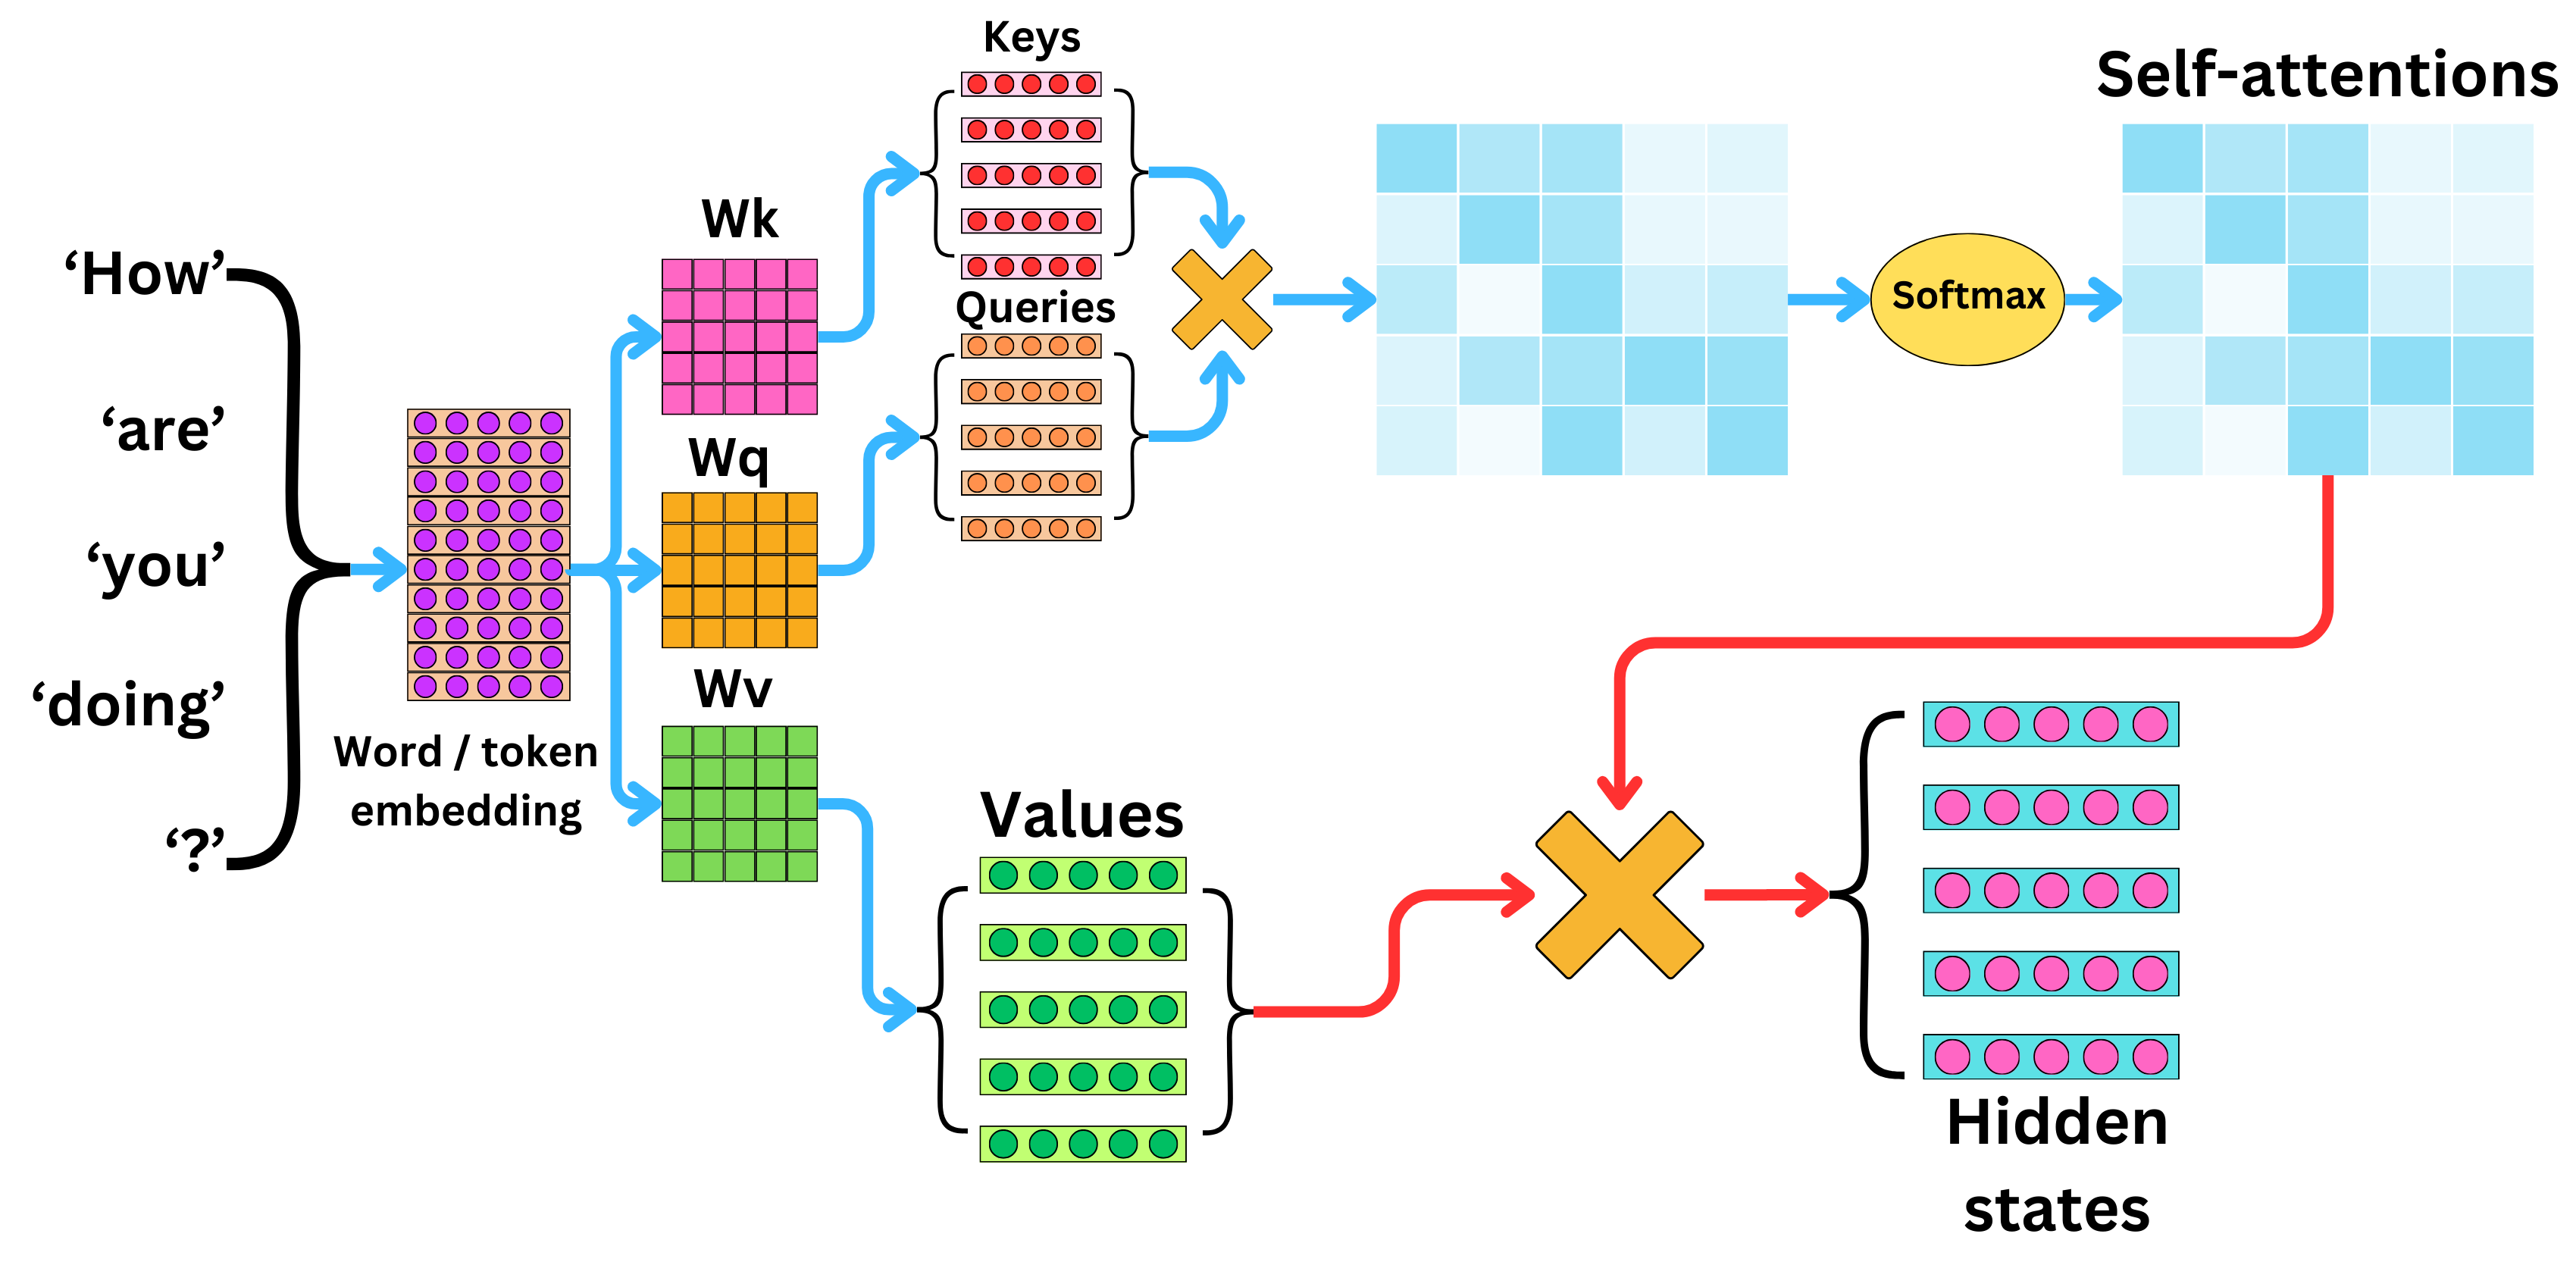
\includegraphics[width=0.8\textwidth]{Images/attention.png}
        \caption{Kiến trúc cơ chế tự chú ý (Self-Attention) trong Transformer \cite{vaswani2017attention}.}
        \label{fig:attetion}
    \end{figure}

    \begin{figure}[H]
        \centering
        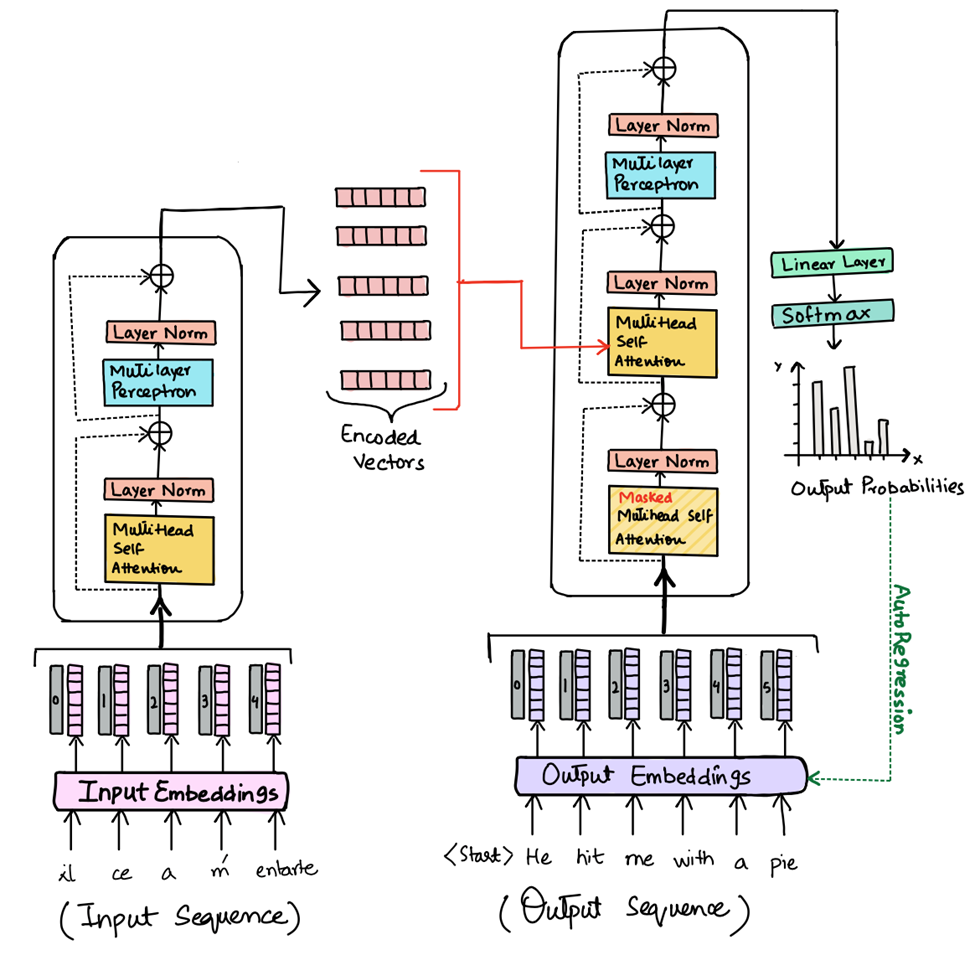
\includegraphics[width=0.8\textwidth]{Images/transformer.png}
        \caption{Kiến trúc tổng thể của Transformer với các lớp Encoder và Decoder \cite{vaswani2017attention}.}
        \label{fig:transformer}
    \end{figure}

\section{Các nghiên cứu liên quan}

\subsection{Tình hình nghiên cứu ngoài nước}
Trên thế giới, bài toán phân tích sắc thái cảm xúc đối với các ngôn ngữ phổ biến đã đạt được rất nhiều thành tựu đáng kể. Phần lớn các nghiên cứu tiên tiến nhất hiện nay đều đã chuyển dịch sang việc áp dụng các mô hình học máy dựa trên kiến trúc Transformer để giải quyết hiệu quả các bài toán phân tích đa miền (multi-domain). Bên cạnh việc tối ưu độ chính xác của mô hình, các nghiên cứu quốc tế cũng đã đề xuất và áp dụng thành công các khung phương pháp luận hệ thống chuyên biệt để xử lý dữ liệu mạng xã hội, bao gồm các bước chuẩn hóa từ việc trích xuất API, tiền xử lý văn bản nhiễu cho đến trực quan hóa kết quả đầu ra.

\subsection{Tình hình nghiên cứu trong nước}
Tại Việt Nam, mặc dù tiếng Việt thuộc nhóm 20 ngôn ngữ có quy mô cộng đồng sử dụng lớn nhất thế giới, các nghiên cứu về phân tích cảm xúc hiện nay phần lớn vẫn chỉ tập trung vào các tập dữ liệu ngách thuộc một miền (domain) cụ thể. Trọng tâm của các công trình nghiên cứu chuyên biệt về văn bản tiếng Việt chủ yếu tập trung vào việc cải tiến cấu trúc các mô hình học máy để tối ưu hóa các chỉ số định lượng (như Accuracy, F1-score) trên các bộ dữ liệu mẫu (benchmark datasets).

Tuy nhiên, xu hướng này dẫn đến một hạn chế lớn là chưa chú trọng đúng mức đến việc xây dựng một quy trình xử lý chuẩn hóa có tính thích ứng cao. Hệ quả là các mô hình thường đạt hiệu suất tốt trong môi trường thực nghiệm nhưng lại bộc lộ nhiều điểm yếu về tính linh hoạt khi triển khai trên dữ liệu thực tế – nơi ngôn ngữ biến đổi liên tục và có độ nhiễu cao như bình luận trên YouTube. Ngoài ra, tiếng Việt còn đối mặt với nhiều thách thức đặc thù về ngôn ngữ chưa được giải quyết triệt để như sự khác biệt phương ngữ, hiện tượng trộn mã (code-switching), hệ thống từ Hán - Việt mang sắc thái tu từ riêng, và sự thiếu phân biệt thị giác giữa các từ đồng âm khác nghĩa do đặc trưng của chữ Quốc ngữ.

\subsection{Tổng hợp và nhận định nghiên cứu}

\chapter{XÂY DỰNG KHUNG PHƯƠNG PHÁP}
\label{Chapter3}

\section{}

\chapter{THỰC NGHIỆM VÀ ĐÁNH GIÁ KẾT QUẢ NGHIÊN CỨU}
\label{Chapter4}

\section{Quy trình thực nghiệm}
Toàn bộ quy trình triển khai và đánh giá thực nghiệm tất cả các khâu trong khung phương pháp (framework) đều được lập trình bằng ngôn ngữ Python, kết hợp cùng framework học sâu PyTorch và thư viện mã nguồn mở Transformers (Hugging Face).

Về môi trường phần cứng, quá trình huấn luyện và kiểm thử các mô hình (\textbf{mBERT}, \textbf{PhoBERT} và \textbf{mModernBERT}) được thực hiện trên hệ thống máy chủ hiệu năng cao. Hệ thống này được trang bị vi xử lý CPU Intel Xeon® E5-2686 v4 (72 cores), dung lượng bộ nhớ trong (RAM) lên đến 258 GB, cùng bộ xử lý đồ họa (GPU) NVIDIA GeForce RTX 3090 sở hữu 24GB VRAM (năng lực tính toán đạt 35.3 TFLOPS), đảm bảo khả năng xử lý song song khối lượng dữ liệu lớn.

Đối với khâu chuẩn bị dữ liệu, tập ngữ liệu sau khi trải qua quá trình gán nhãn và giảm mẫu đa số (Undersampling) được phân chia ngẫu nhiên thành ba tập con độc lập: tập huấn luyện (Training set), tập kiểm định (Validation set) và tập kiểm thử (Test set) với tỷ lệ phân bổ tương ứng là 90:5:5.

Về quá trình huấn luyện, cấu hình của ba mô hình được thiết lập chi tiết dựa trên các siêu tham số trình bày tại Bảng \ref{tab:hyperparameters_detail}. Nhằm tối ưu hóa thời gian tính toán và ngăn chặn hiện tượng quá khớp (overfitting), kỹ thuật dừng sớm (Early Stopping) được tích hợp vào quy trình. Cụ thể, tiến trình huấn luyện sẽ tự động chấm dứt nếu độ đo hiệu năng trên tập kiểm định không ghi nhận sự cải thiện nào sau hai chu kỳ (epochs) liên tiếp.

\begin{table}[H]
    \centering
    \renewcommand{\arraystretch}{1.5} 
    \caption{Cấu hình siêu tham số chi tiết cho từng mô hình thực nghiệm.}
    \label{tab:hyperparameters_detail}
    \begin{tabular}{|p{5.5cm}|c|c|c|}
        \hline
        \textbf{Siêu tham số} & \textbf{mBERT} & \textbf{PhoBERT} & \textbf{mModernBERT} \\
        \hline
        Số lượng nhãn phân loại (\textit{n\_classes}) & 28 & 28 & 28 \\
        \hline
        Độ dài chuỗi tối đa (\textit{max\_len}) & 512 & \textbf{256} & 512 \\
        \hline
        Hệ số học (\textit{learning rate}) & $2.0 \times 10^{-5}$ & $2.0 \times 10^{-5}$ & $\mathbf{1.0 \times 10^{-5}}$ \\
        \hline
        Số vòng huấn luyện (\textit{epochs}) & 12 & 12 & 12 \\
        \hline
        Kích thước lô (\textit{batch\_size}) & 32 & 32 & 32 \\
        \hline
        Tích lũy gradient (\textit{accumulate\_steps}) & 2 & 2 & 2 \\
        \hline
        Kích thước lô hiệu dụng (\textit{effective batch}) & 64 & 64 & 64 \\
        \hline
        Tỷ lệ Dropout & 0.1 & 0.1 & 0.1 \\
        \hline
        Độ chính xác hỗn hợp (\textit{FP16}) & Có & Có & Có \\
        \hline
        Tham số $\beta$ (CB-Loss) & 0.999 & 0.999 & 0.999 \\
        \hline
        Số lượng khoảng (\textit{GHM bins}) & 10 & 10 & 10 \\
        \hline
    \end{tabular}
\end{table}

\section{Kết quả thực nghiệm}

\subsection{Kết quả quá trình thu thập, xây dựng, tiền xử lý và gán nhãn dữ liệu}
Thông qua các biểu đồ phân phối tập dữ liệu sau quá trình thu thập và xây dựng, tiền xử lý (Hình \ref{fig:first_cbc} và Hình \ref{fig:first_vbc}) đều có thể thấy được tập ngữ liệu mang đặc tính mất cân bằng sâu sắc mang tính tự nhiên (Long-tail distribution). Các chủ đề mang tính thời sự hoặc giải trí cao (như \texttt{news}, \texttt{music}) thu hút lượng tương tác áp đảo, trong khi các danh mục khác lại vô cùng hạn chế. Sự phân bố không cân bằng này chính là minh chứng cho thấy nếu sử dụng phương pháp luận truyền thống, mô hình sẽ hoàn toàn bị thiên kiến (bias) theo các chủ đề phổ biến. Do đó, việc framework tích hợp \textbf{cơ chế gán nhãn bán tự động} (kết hợp luật từ vựng và sinh dữ liệu nhân tạo) cùng \textbf{hàm mất mát hỗn hợp (Mixture Loss)} là một bước đi mang tính chiến lược và bắt buộc.

\begin{figure}[H]
    \centering
    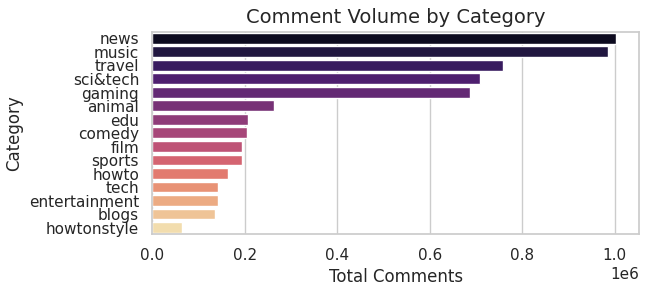
\includegraphics[width=0.8\textwidth]{Images/comment_by_cate.png}
    \caption{Phân phối dữ liệu số lượng bình luận sau quá trình thu thập và tiền xử lý theo các danh mục.}
    \label{fig:first_cbc}
    \vspace{0.1cm}
\end{figure}

\begin{figure}[H]
    \centering
    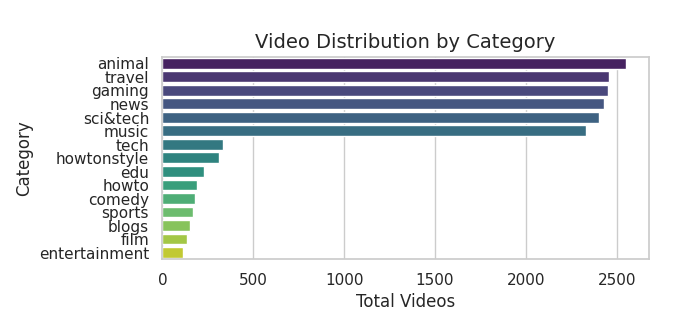
\includegraphics[width=0.8\textwidth]{Images/vid_by_cate.png}
    \caption{Phân phối dữ liệu số lượng video sau quá trình thu thập và tiền xử lý theo các danh mục.}
    \label{fig:first_vbc}
    \vspace{0.1cm}
\end{figure}

Biểu đồ violin (Hình \ref{fig:first_cmt_violin}) chỉ ra rằng tuyệt đại đa số bình luận của người dùng mạng xã hội Việt Nam thường có độ dài vô cùng ngắn (tập trung ở ngưỡng dưới 20 từ, kể cả icons). Việc phân loại cảm xúc vi mô (fine-grained emotions) trên các đoạn văn bản thiếu hụt ngữ cảnh trầm trọng là một thách thức cực đại đối với học máy. Tuy nhiên, giới hạn này lại làm nổi bật tính đúng đắn trong việc lựa chọn và thiết kế framework. Nhờ việc tinh chỉnh các \textbf{kiến trúc Transformer tiên tiến (như mModernBERT với cơ chế Attention tối ưu)}, framework có đủ độ nhạy bén để trích xuất các dấu hiệu ngữ nghĩa tinh tế nhất chỉ từ một vài từ khóa, vượt qua rào cản về độ dài văn bản mà các mô hình biểu diễn ngữ nghĩa truyền thống thường thất bại.
Ngoài ra, sự xuất hiện của các điểm dị thường (outliers) kéo dài lên tới 250 tokens cho thấy độ nhiễu và tính đa dạng hóa của tập ngữ liệu.

\begin{figure}[H]
    \centering
    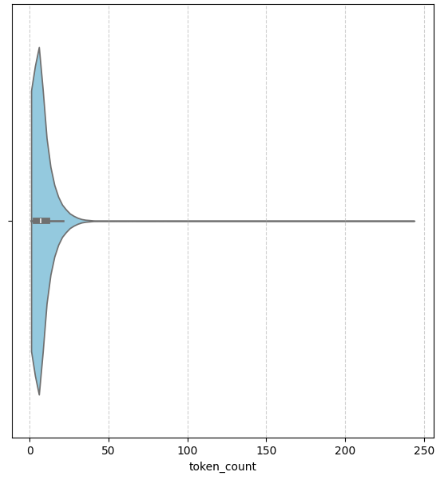
\includegraphics[width=0.8\textwidth]{Images/stats_tk.png}
    \caption{Biểu đồ violin phân phối số lượng từ trong từng bình luận.}
    \label{fig:first_cmt_violin}
    \vspace{0.1cm}
\end{figure}

Kết quả của quá trình gán nhãn bán tự động được thể hiện qua phân phối dữ liệu dựa theo các nhóm cảm xúc (Hình \ref{fig:label_anno_dist}) bộc lộ rõ rệt cấu trúc phân phối đuôi dài (long-tail distribution) mang tính tự nhiên. Các nhãn thuộc nhóm tích cực áp đảo hoàn toàn các nhãn thuộc nhóm tiêu cực. Đồng thời, việc số lượng nhãn trung tính (neutral) đột biến lại là một tín hiệu tốt và mang tính bảo chứng. Vì thực tế trên mạng xã hội (YouTube, TikTok, Facebook), 70\% - 80\% bình luận thực tế là vô thưởng vô phạt, ngắn gọn, hoặc thuần túy trần thuật (ví dụ: "video hay", "chấm", "đã xem", "ông A đi xe màu đỏ").

Đồng thời, bức tranh phân bố cảm xúc cũng cho thấy sự tương đồng với tập dữ liệu GoEmotions đã được kiểm chứng nghiêm ngặt (như Hình \ref{fig:label_goemo_dist}). Sự nhất quán về mặt phân phối này khẳng định rằng sự kết hợp giữa luật từ vựng (rule-based) và mô hình ngôn ngữ (Encoder) trong khung phương pháp đã thành công trong việc chuyển giao tri thức (knowledge transfer) từ chuyên gia con người sang hệ thống máy tính với độ sai số được kiểm soát chặt chẽ.

\begin{figure}[H]
    \centering
    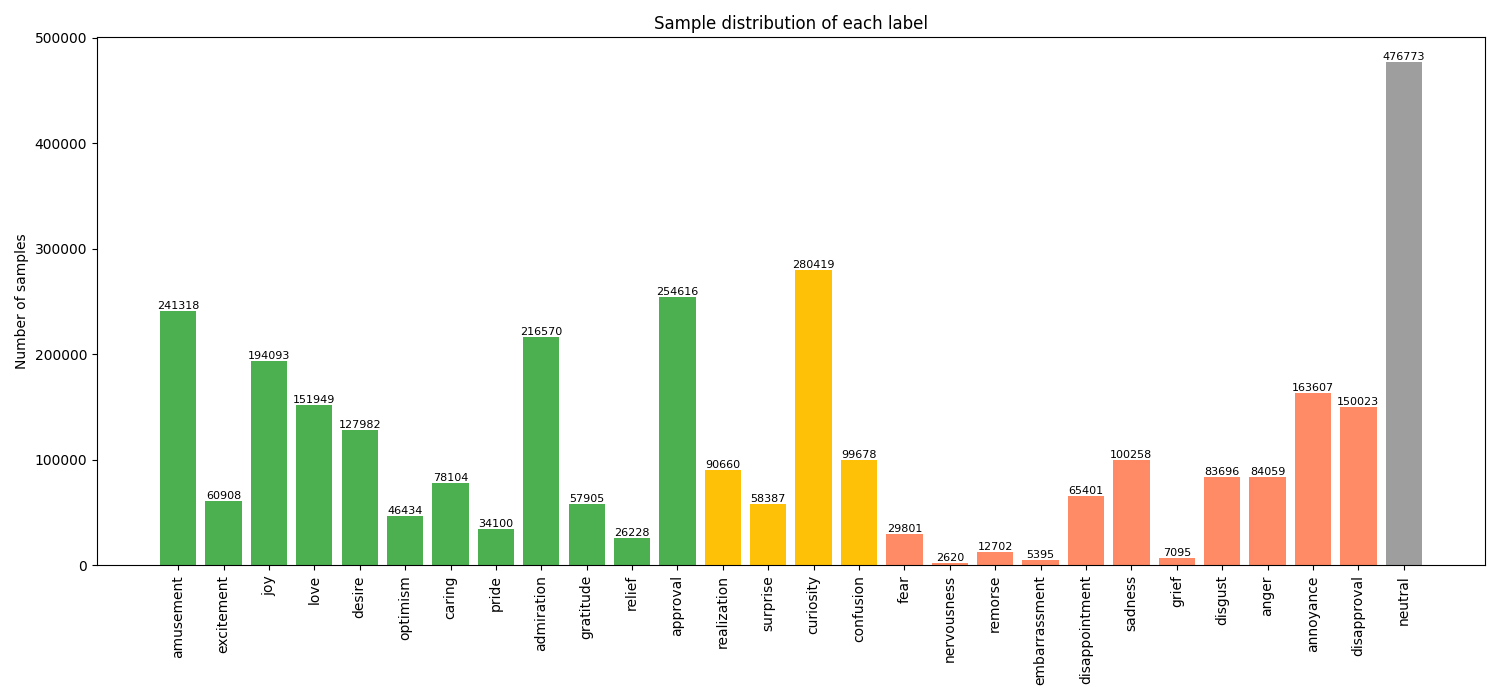
\includegraphics[width=0.8\textwidth]{Images/label_distribution.png}
    \caption{Biểu đồ phân phối dữ liệu theo các nhóm cảm xúc (xanh - tích cực, đỏ - tiêu cực, vàng - nhập nhằng, xám - trung tính) sau khi được gán nhãn.}
    \label{fig:label_anno_dist}
    \vspace{0.1cm}
\end{figure}

\begin{figure}[H]
    \centering
    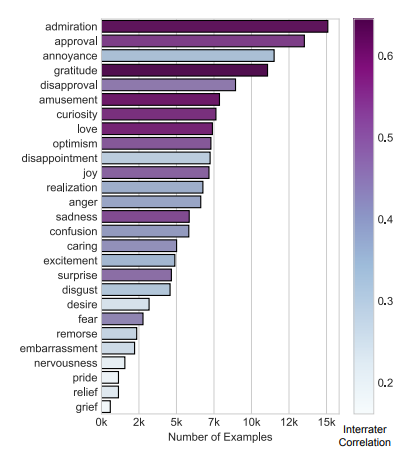
\includegraphics[width=0.8\textwidth]{Images/goemo_labeldist.png}
    \caption{Biểu đồ phân phối dữ liệu theo các cảm xúc vi mô trong tập GoEmotions.}
    \label{fig:label_goemo_dist}
    \vspace{0.1cm}
    {\small Nguồn: \parencite{demszky2020goemotions}}
\end{figure}

\subsection{Kết quả quá trình huấn luyện mô hình}
\begin{figure}[H]
    \centering
    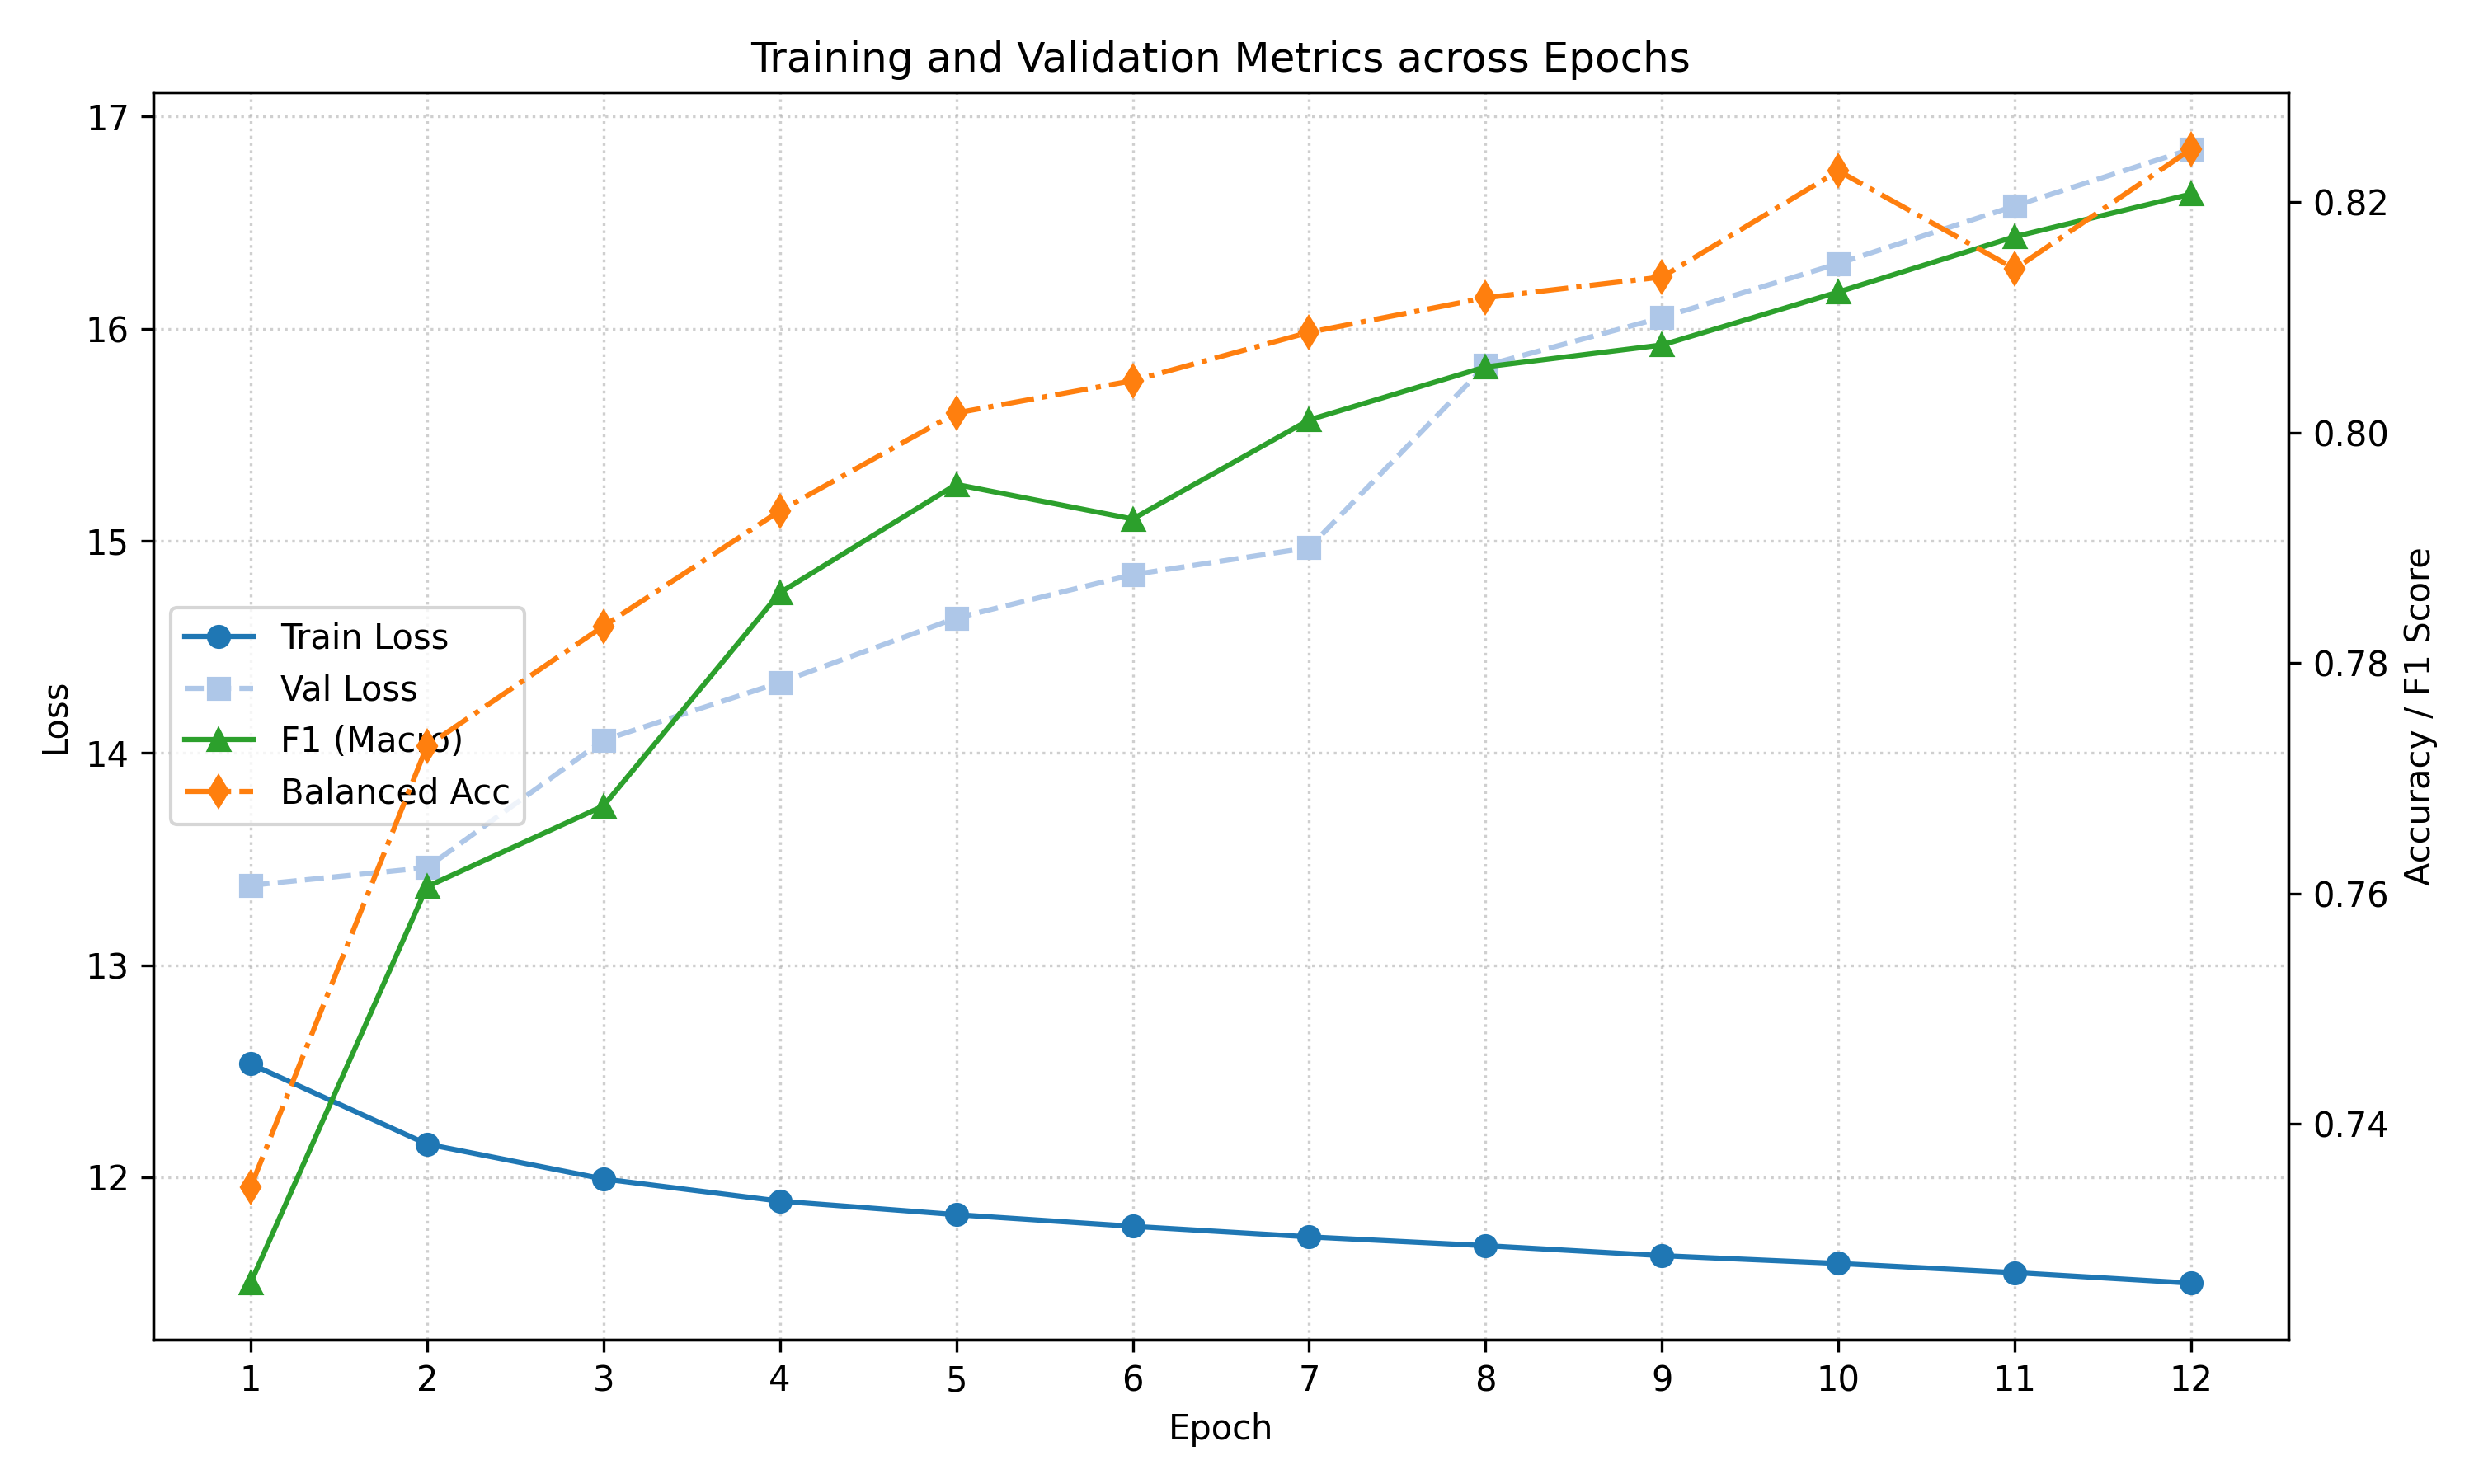
\includegraphics[width=0.8\textwidth]{Images/eps_mbert.png}
    \caption{Biểu đồ hành vi trong quá trình hiệu chỉnh mô hình mBERT.}
    \label{fig:eps_mbert}
    \vspace{0.1cm}
\end{figure}

\begin{figure}[H]
    \centering
    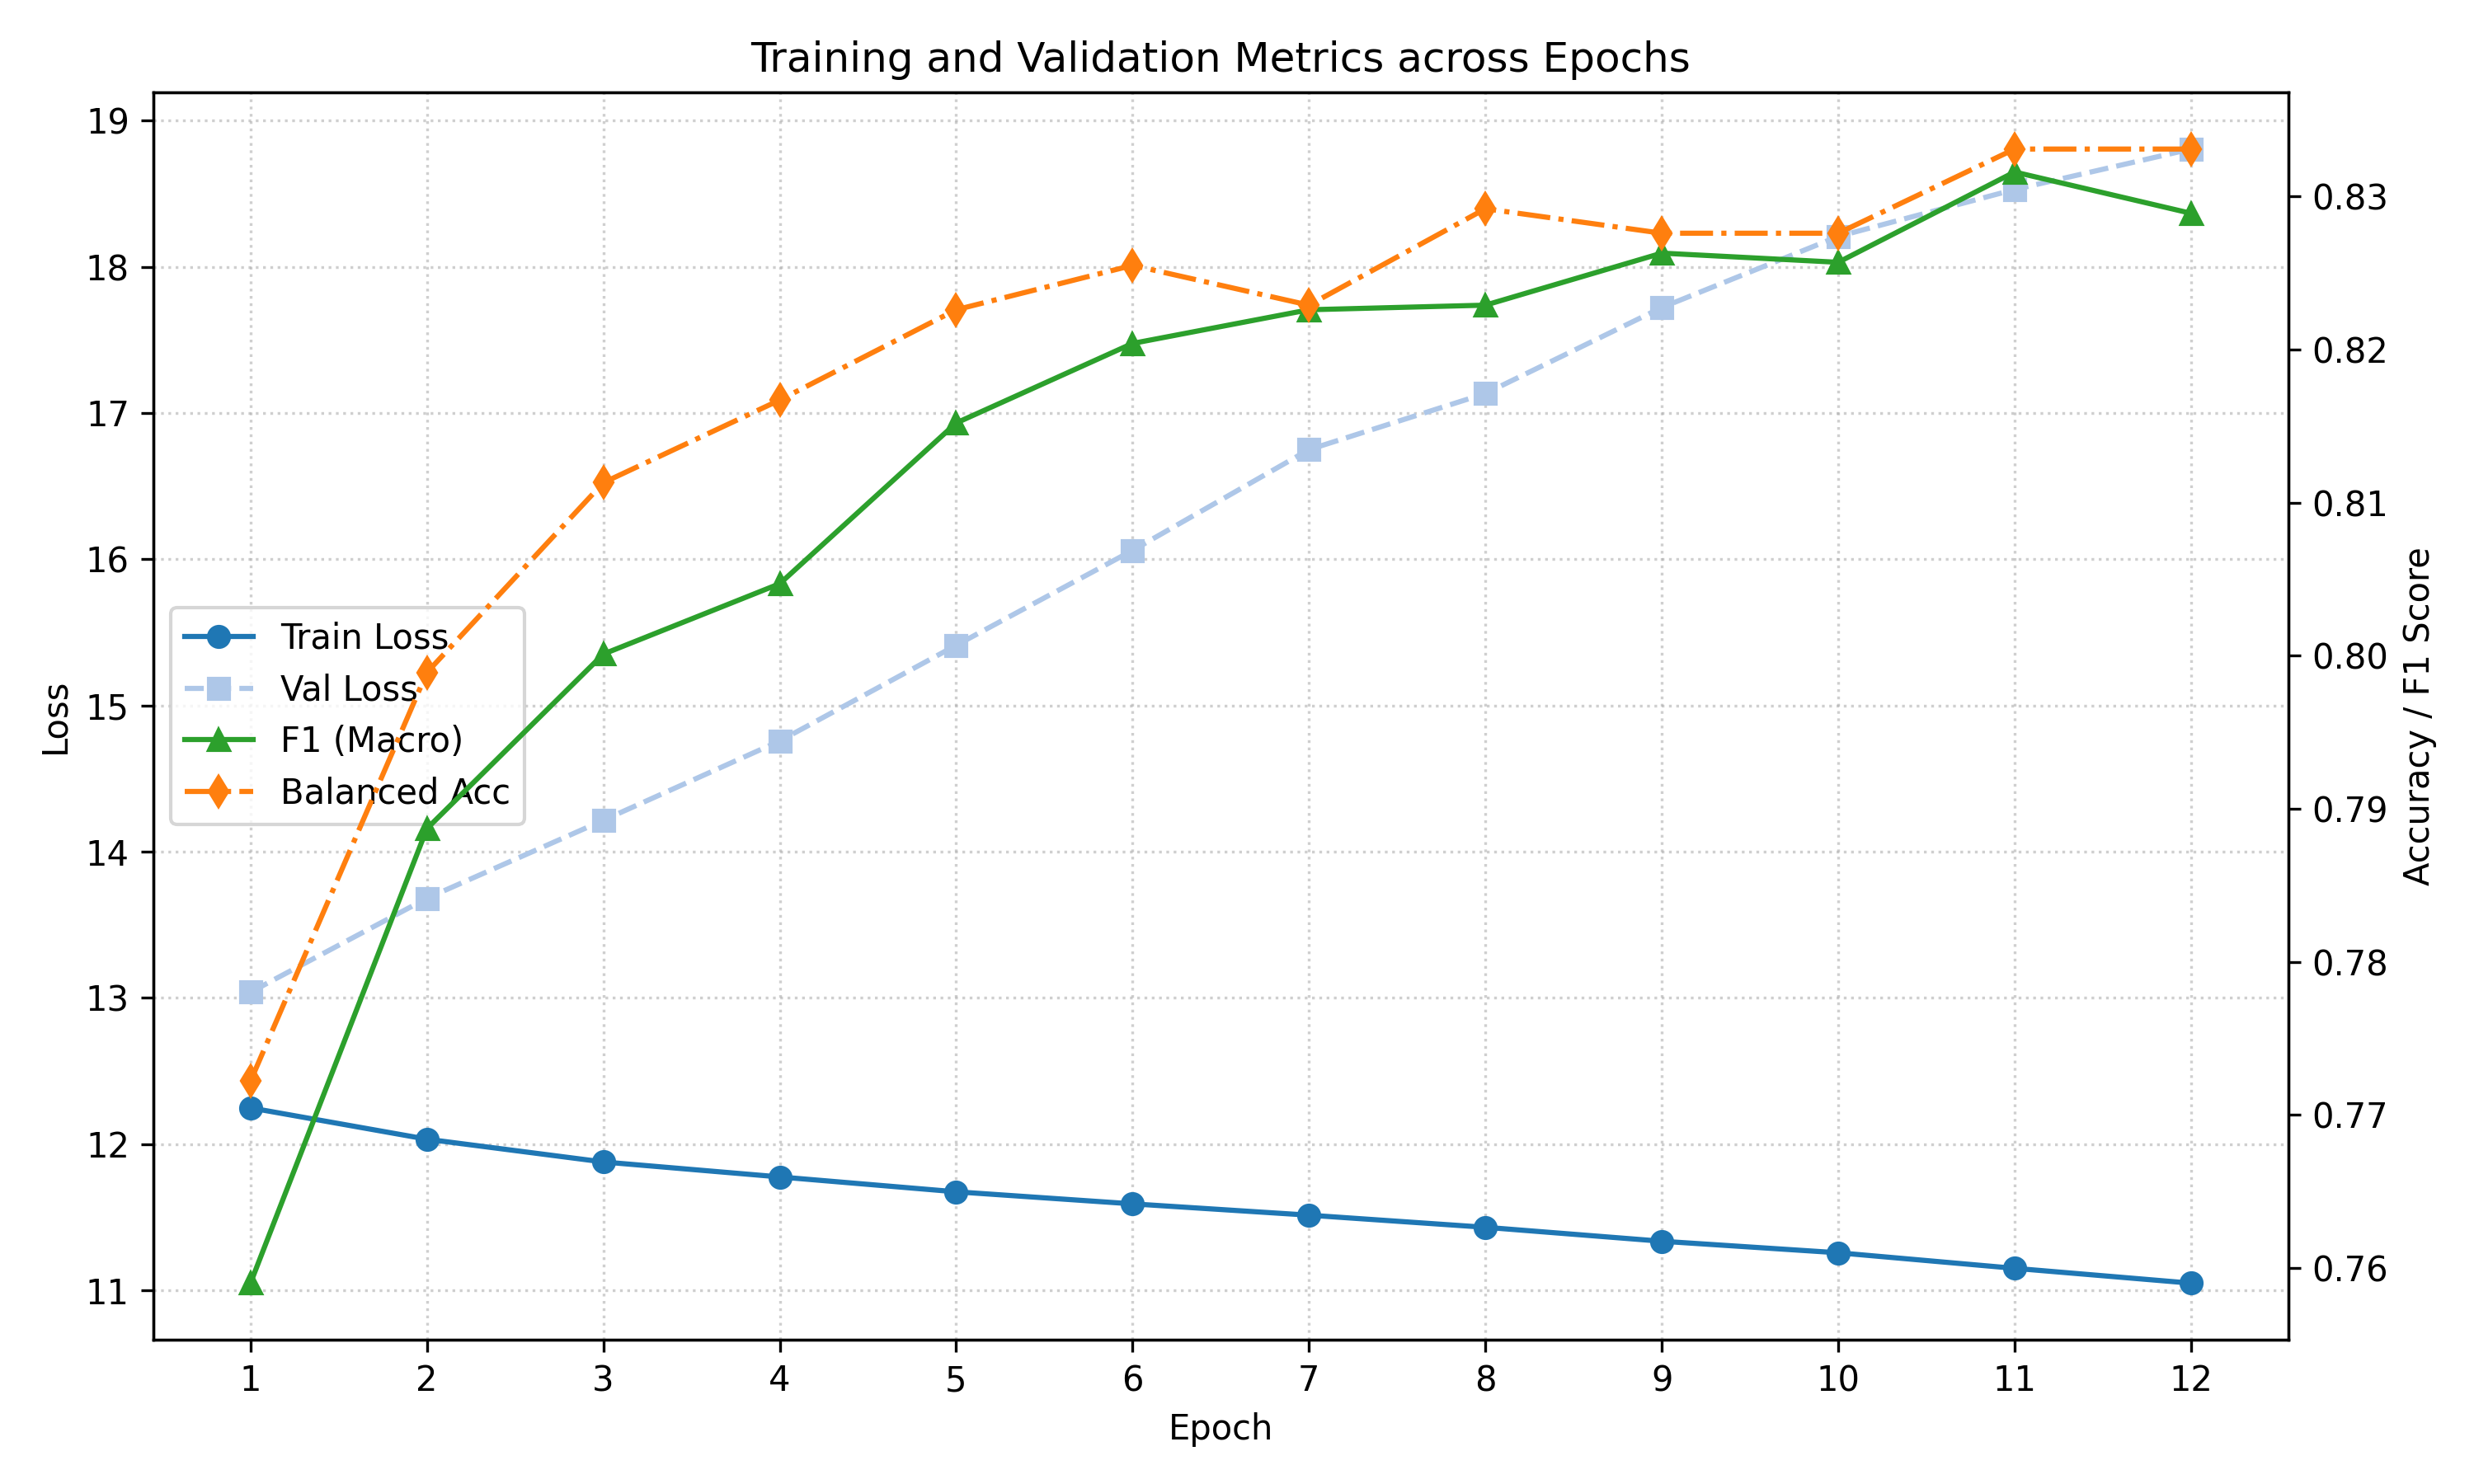
\includegraphics[width=0.8\textwidth]{Images/eps_phobert.png}
    \caption{Quá trình hiệu chỉnh mô hình phoBERT.}
    \label{fig:eps_phobert}
    \vspace{0.1cm}
\end{figure}

\begin{figure}[H]
    \centering
    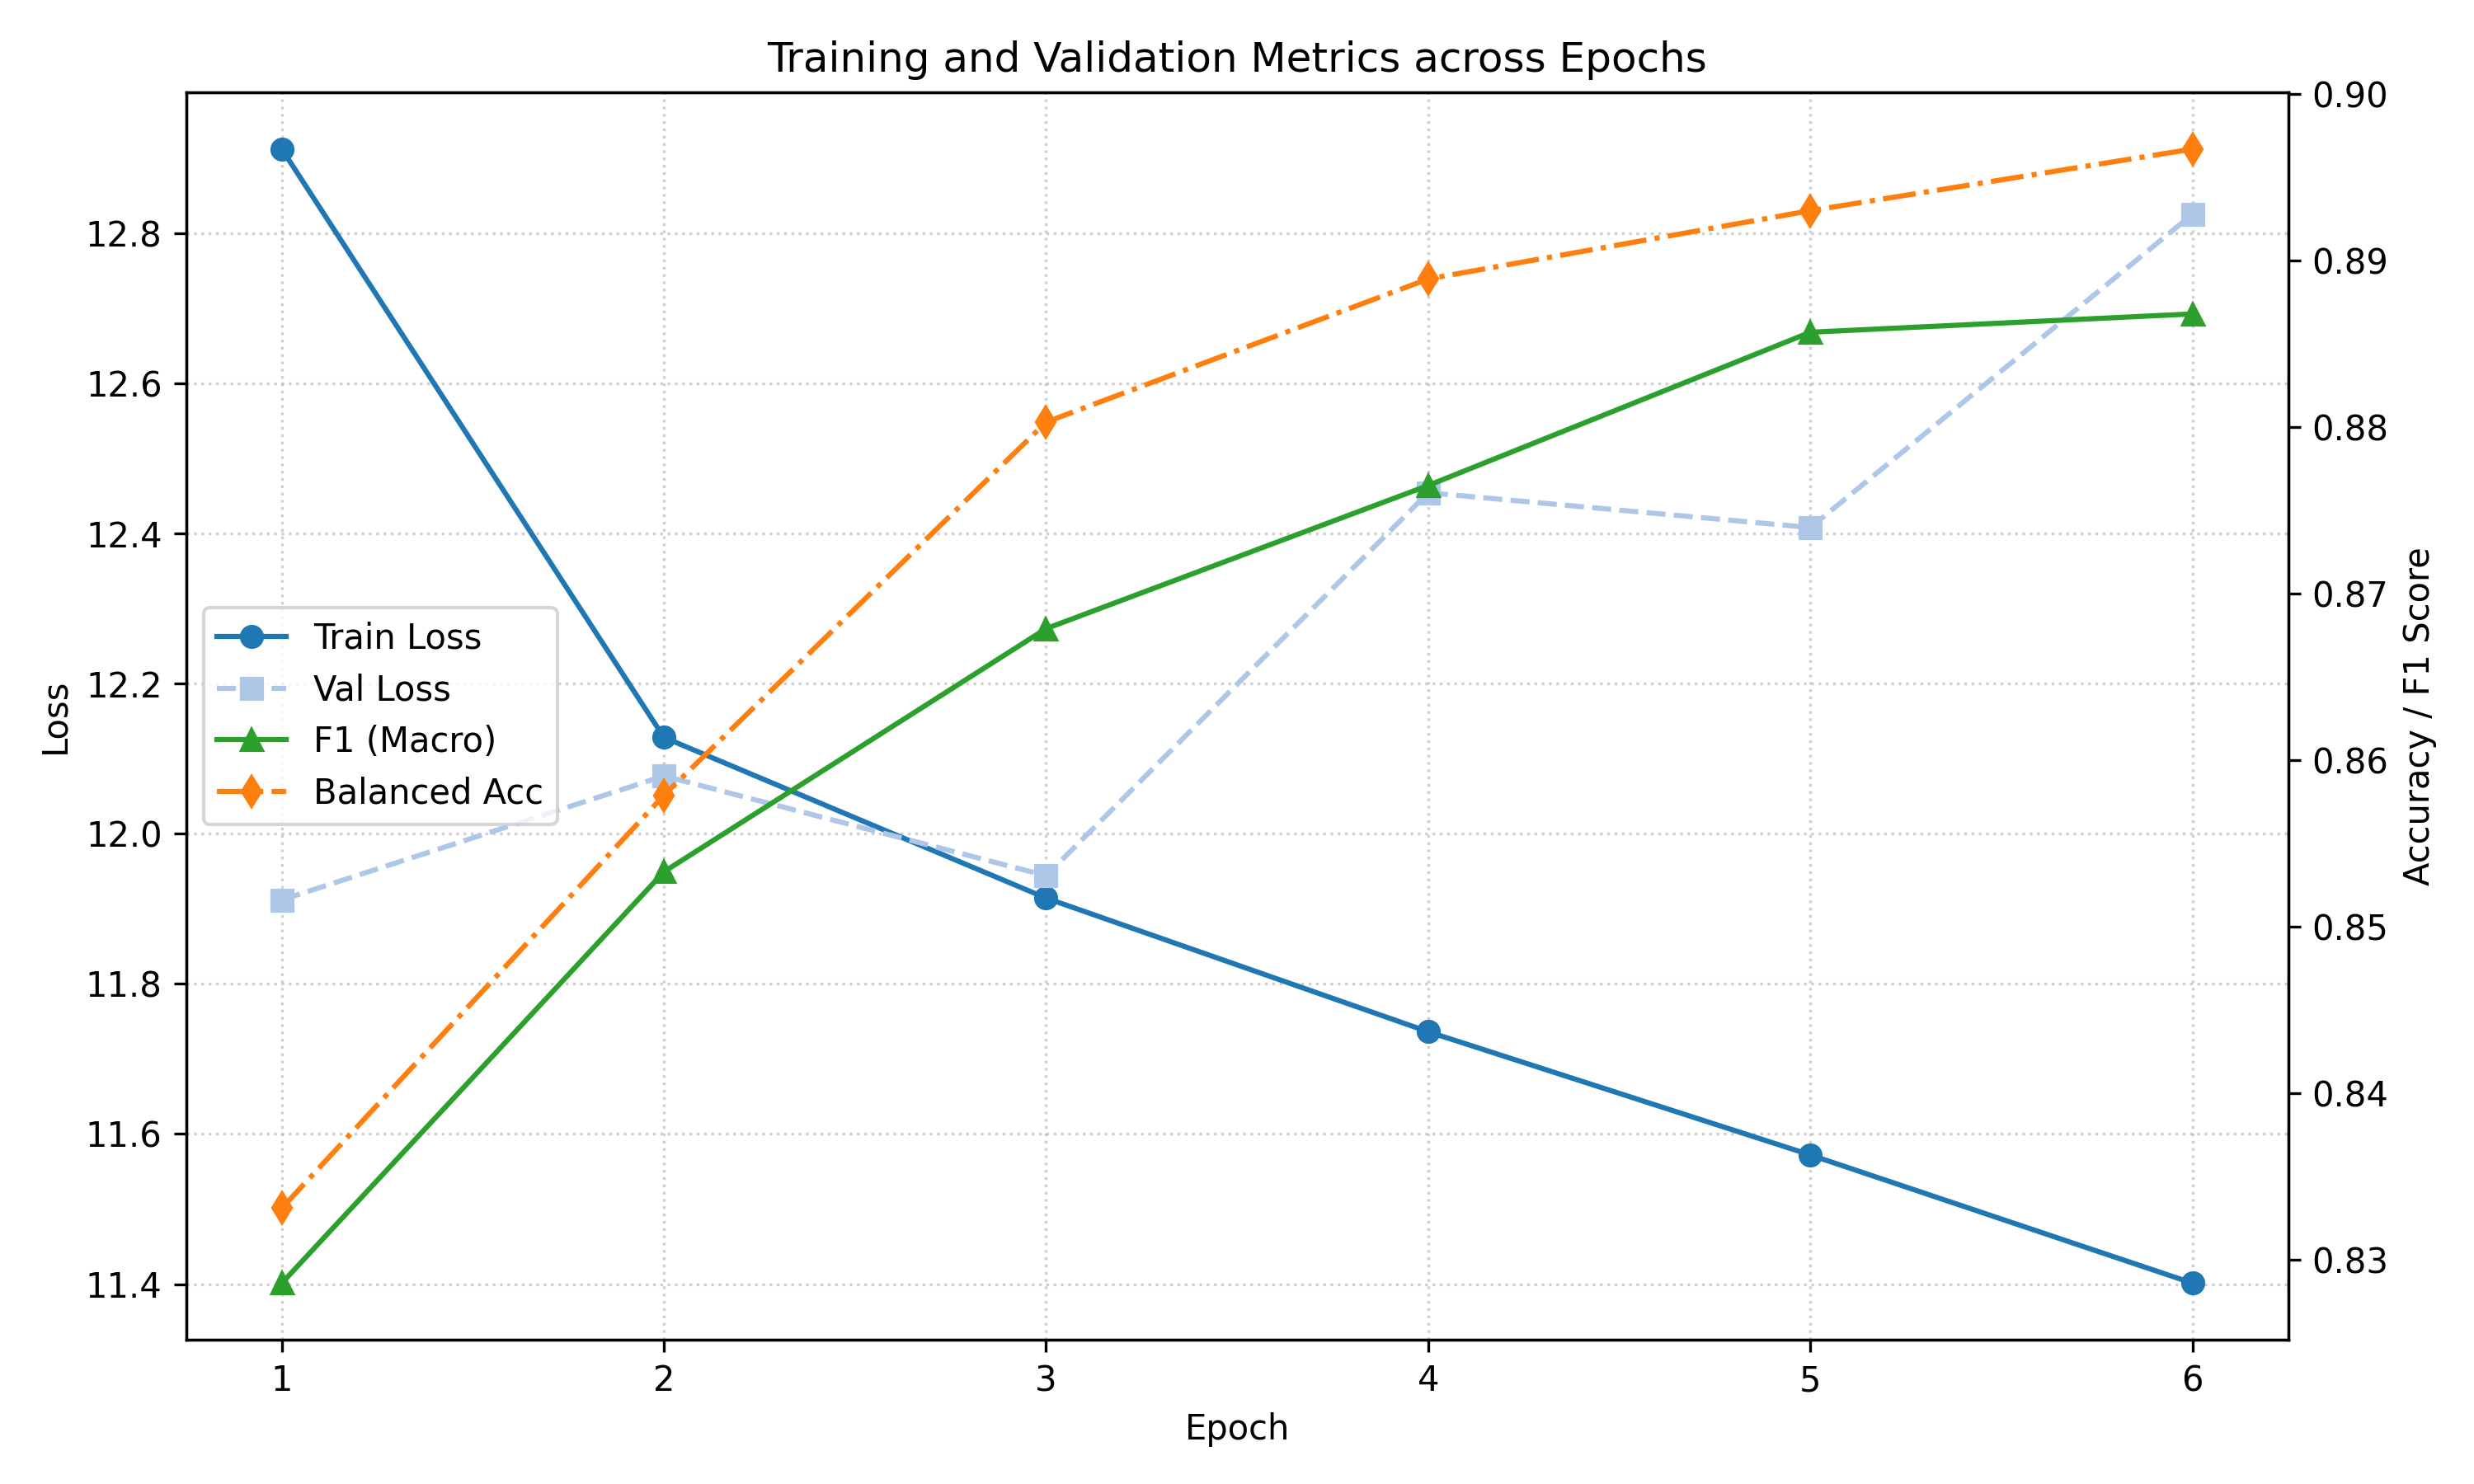
\includegraphics[width=0.8\textwidth]{Images/eps_mmbert.png}
    \caption{Quá trình hiệu chỉnh mô hình mModernBERT.}
    \label{fig:eps_modernbert}
    \vspace{0.1cm}
\end{figure}

Từ ba biểu đồ quá trình huấn luyện trên tập dữ liệu lớn với gần 3 triệu điểm dữ liệu và trên 28 lớp không cân bằng (imbalance) (Hình \ref{fig:eps_mbert}, Hình \ref{fig:eps_phobert} và Hình \ref{fig:eps_modernbert}) cho thấy hiện tượng phân kỳ sớm của giá trị mất mát kiểm định. Tuy nhiên, nếu ta đi vào phân tích sâu hơn, thì có thể nhận thấy rằng đây hoàn toàn là đặc trưng toán học mong muốn khi kết hợp giữa CB-Loss và GHM Loss nhằm bảo vệ các lớp thiểu số.

Đồng thời, hiệu năng thực tế của mô hình (thể hiện qua F1-Macro và Balanced Accuracy) vẫn không hề suy giảm mà vẫn tăng trưởng ổn định. Đặc biệt, các kết quả cũng cho thấy rằng điểm dừng lý tưởng (Early Stopping) rơi vào khoảng 3-5 epoch đầu tiên.


\subsection{Kết quả quá trình kiểm thử mô hình}

\begin{table}[H]
    \centering
    \renewcommand{\arraystretch}{1.3} 
    \caption{Kết quả đánh giá hiệu năng tổng thể của các mô hình trên tập kiểm thử.}
    \label{tab:overall_results}
    \begin{tabular}{|l|c|c|c|}
        \hline
        \textbf{Mô hình} & \textbf{F1-Macro} & \textbf{Overall Accuracy} & \textbf{Balanced Accuracy} \\
        \hline
        mBERT & $82.19 \pm 0.38\%$ & $82.93 \pm 0.19\%$ & $82.35 \pm 0.44\%$ \\
        \hline
        PhoBERT & $82.99 \pm 0.36\%$ & $83.84 \pm 0.18\%$ & $82.99 \pm 0.43\%$ \\
        \hline
        \textbf{mModernBERT} & $\mathbf{88.94 \pm 0.34\%}$ & $\mathbf{91.53 \pm 0.14\%}$ & $\mathbf{89.80 \pm 0.38\%}$ \\
        \hline
    \end{tabular}
\end{table}

Kết quả từ Bảng \ref{tab:overall_results} cho thấy mô hình \textbf{mModernBERT} đạt hiệu năng cao nhất trên toàn bộ các thang đo, bỏ xa hai mô hình còn lại. Với chỉ số F1-Macro đạt $88.94\%$ và độ chính xác tổng thể (Overall Accuracy) lên tới $91.53\%$, mModernBERT chứng minh khả năng biểu diễn ngôn ngữ vượt trội. Sự chênh lệch này có thể được lý giải bởi các cải tiến kiến trúc cốt lõi của ModernBERT, bao gồm cơ chế mã hóa vị trí tương đối RoPE (Rotary Position Embedding) và khả năng xử lý ngữ cảnh dài. Những cải tiến này giúp mô hình nắm bắt tốt hơn cấu trúc ngữ pháp lỏng lẻo và các phụ tố cảm xúc phức tạp đặc trưng của ngôn ngữ mạng xã hội.

Khi đối chiếu giữa mBERT và PhoBERT, có thể thấy PhoBERT mang lại kết quả nhỉnh hơn ở cả ba độ đo (F1-Macro đạt $82.99\%$ so với $82.19\%$ của mBERT). Mặc dù có cùng chung nền tảng kiến trúc Encoder cơ sở, PhoBERT được hưởng lợi lớn từ việc tiền huấn luyện (pre-training) hoàn toàn trên ngữ liệu tiếng Việt khổng lồ, kết hợp cùng cơ chế phân đoạn từ (word segmentation).

Một điểm sáng cực kỳ quan trọng trong Bảng \ref{tab:overall_results} là sự đồng đều giữa các độ đo \textbf{Overall Accuracy} và \textbf{F1-Macro / Balanced Accuracy}. Thông thường, trên một tập dữ liệu phân phối đuôi dài , một mô hình kém sẽ có Overall Accuracy rất cao (do đoán bừa nhãn đa số) nhưng F1-Macro lại sụt giảm nghiêm trọng. Tuy nhiên, ở đây chỉ số F1-Macro và Balanced Accuracy của cả ba mô hình đều duy trì ở mức $>82\%$ (riêng mModernBERT tiệm cận $90\%$). Kết quả này là bảo chứng mạnh mẽ nhất cho thấy việc kết hợp kỹ thuật giảm mẫu (Undersampling) và hàm điều chuẩn \textbf{Mixture Loss (CB-Loss + GHM-Loss)} đã phát huy tác dụng triệt để. Mô hình không bị rơi vào hiện tượng quá khớp với nhãn đa số mà thực sự học được cách phân loại các nhãn cảm xúc thiểu số một cách công bằng.

Độ lệch chuẩn (standard deviation - các giá trị $\pm$) thu được từ quá trình đánh giá chéo trên các thang đo đều duy trì ở mức rất thấp, dao động trong khoảng từ $0.14\%$ đến $0.44\%$. Phương sai nhỏ này minh chứng cho tính ổn định (robustness) của hệ thống trong suốt quá trình học. Các mô hình đã hội tụ tốt, không bị nhạy cảm (sensitive) với các thay đổi ngẫu nhiên của các lô dữ liệu (batch) và có khả năng tổng quát hóa (generalization) cao khi đối mặt với dữ liệu chưa từng thấy trong tập kiểm thử.

\chapter{KẾT LUẬN VÀ HƯỚNG PHÁT TRIỂN}
\label{Chapter5}

\section{Kết luận chung}
Nghiên cứu đã xây dựng và kiểm chứng thành công một khung phương pháp toàn diện, bao quát trọn vẹn các bước từ thu thập dữ liệu, tiền xử lý, gán nhãn cho đến tinh chỉnh mô hình, nhằm giải quyết bài toán phân loại cảm xúc vi mô trên ngữ liệu mạng xã hội tiếng Việt. Giá trị cốt lõi của khung phương pháp này là khả năng xử lý triệt để những thách thức đặc thù của dữ liệu thực tế như văn bản thiếu ngữ cảnh, độ nhiễu cao và sự mất cân bằng trong phân phối. Việc chuẩn hóa quy trình không chỉ giúp tối ưu nguồn lực tính toán, mà còn tạo dựng một hệ thống linh hoạt, có khả năng mở rộng cho các bài toán phân tích ngữ nghĩa phức tạp hơn. Trên cơ sở lý thuyết cùng các minh chứng thực nghiệm định lượng, nghiên cứu rút ra những kết luận chính như sau.

\textbf{Thứ nhất, về tính thực tiễn của quy trình gán nhãn bán tự động:} Việc kết hợp tập luật từ vựng (rule-based) với các Mô hình Ngôn ngữ Lớn (LLMs) dựa trên tập hạt giống (seed data) đã cho thấy hiệu quả vượt trội, giải quyết thành công bài toán thời gian và chi phí vốn là điểm yếu của phương pháp gán nhãn chuyên gia truyền thống khi xử lý dữ liệu quy mô lớn. Đáng chú ý, phân phối nhãn thu được phản ánh trung thực cấu trúc đuôi dài tự nhiên của ngôn ngữ mạng xã hội, vừa đảm bảo độ chính xác vừa hạn chế tối đa tình trạng gán nhãn sai cho các nhóm cảm xúc thiểu số.

\textbf{Thứ hai, về năng lực mô hình và kỹ thuật xử lý mất cân bằng dữ liệu:} Kết quả thực nghiệm cho thấy ưu thế rõ rệt của kiến trúc \textbf{mModernBERT}, nhờ những cải tiến trong cơ chế Attention và khả năng mở rộng ngữ cảnh, mô hình đạt chỉ số F1-Macro vượt quá $88\%$. Thành tựu này phần lớn đến từ chiến lược xử lý mất cân bằng dữ liệu: kết hợp kỹ thuật giảm mẫu đa số với hàm mất mát hỗn hợp \textbf{Mixture Loss} (gồm CB-Loss và GHM-Loss), giúp điều chỉnh hiệu quả trọng số học tập của mô hình. Nhờ đó, hệ thống không bị chi phối bởi các nhãn phổ biến mà vẫn giữ được độ nhạy cao với những cảm xúc tiêu cực vi mô hiếm gặp như sợ hãi (\texttt{fear}), hối tiếc (\texttt{remorse}) hay thương tiếc (\texttt{grief}).

\textbf{Tóm lại,} sự kết hợp chặt chẽ giữa quy trình tự động hóa dữ liệu và các kỹ thuật điều chỉnh mô hình chuyên sâu đã chứng minh được tính chính xác, độ tin cậy và toàn diện của khung phương pháp đề xuất. Nghiên cứu không chỉ mang lại một giải pháp học máy tối ưu cho việc Phân tích Cảm xúc tiếng Việt, mà còn khẳng định ứng dụng vào thực tiễn mạnh mẽ, tạo nền tảng để triển khai các hệ thống lắng nghe xã hội (social listening) và giám sát dư luận tự động với độ chính xác cao.

\section{Hướng phát triển}

Mặc dù khung phương pháp đề xuất đã đạt nhiều kết quả khả quan trong thực nghiệm và cho thấy được tính khả thi, một số giới hạn vẫn cần được nhìn nhận. Trên cơ sở đó, các hướng nghiên cứu tiếp theo sẽ tập trung hoàn thiện và mở rộng khả năng ứng dụng của hệ thống.

Hiện nay, nghiên cứu vẫn chủ yếu khai thác đặc trưng ngữ nghĩa từ dữ liệu văn bản (text-based), trong khi trên thực tế, cảm xúc người dùng ở các nền tảng mạng xã hội thường chịu ảnh hưởng từ bối cảnh video, hình ảnh hay âm thanh đi kèm. Việc thiếu hụt dữ liệu đa phương thức vì vậy có thể dẫn đến sai lệch khi phân tích những bình luận mang tính châm biếm hoặc sử dụng tiếng lóng phụ thuộc ngữ cảnh.

Bên cạnh đó, dù quy trình tạo nhãn giả (pseudo-labeling) đã được kiểm soát chặt chẽ, việc phụ thuộc vào đầu ra của Mô hình Ngôn ngữ Lớn vẫn tiềm ẩn rủi ro sai sót đối với những trạng thái cảm xúc nằm ở vùng ranh giới.

Ngoài ra, các kiến trúc Transformer cỡ lớn như mModernBERT đòi hỏi tài nguyên phần cứng đáng kể, gây khó khăn về độ trễ khi cần triển khai hệ thống phân tích thời gian thực ở quy mô lớn.

Nhằm khắc phục những hạn chế vừa nêu, các hướng phát triển tiếp theo sẽ tập trung vào:

- Bổ sung thêm luồng dữ liệu âm thanh và video bên cạnh văn bản, nhằm xây dựng một không gian biểu diễn ngữ nghĩa toàn diện hơn, qua đó hỗ trợ tốt hơn cho bài toán nhận diện cảm xúc châm biếm cũng như các bối cảnh còn ẩn khuất.

- Tích hợp cơ chế Học chủ động (Active Learning) vào khung phương pháp, cho phép hệ thống tự động chọn lọc những mẫu dữ liệu mà mô hình dự đoán với độ tin cậy thấp nhất để chuyển cho chuyên gia thẩm định, trước khi cập nhật trở lại tập huấn luyện nhằm cải thiện chất lượng dữ liệu.

- Áp dụng các kỹ thuật như lượng tử hóa (Quantization) hoặc chưng cất tri thức (Knowledge Distillation) nhằm thu gọn kiến trúc mModernBERT thành phiên bản nhẹ hơn, vừa đảm bảo tốc độ suy luận nhanh vừa duy trì hiệu suất phân lớp tốt, phù hợp cho hệ thống giám sát mạng xã hội theo thời gian thực.

- Triển khai thử nghiệm đối sánh hiệu năng giữa hệ thống hiện tại với các hướng tiếp cận dựa trên Prompt Engineering (Few-shot/Zero-shot learning) từ những mô hình sinh tiên tiến, nhằm đánh giá khả năng thay thế hoặc kết hợp trong tương lai.


% Công trình của tác giả (nếu không có thì comment 02 dòng dưới)
%\addcontentsline{toc}{chapter}{Danh mục công trình của tác giả}
%\include{Appendix/publish}

% In tài liệu tham khảo
\clearpage
\phantomsection
\addcontentsline{toc}{chapter}{DANH MỤC TÀI LIỆU THAM KHẢO}
\printbibheading[title={DANH MỤC TÀI LIỆU THAM KHẢO}]

\printbibliography[heading=subbibliography, title={Tiếng Việt}, keyword=Viet, resetnumbers=true]

\DeclareNameAlias{sortname}{family-given}
\DeclareNameAlias{default}{family-given}

\printbibliography[heading=subbibliography, title={Tiếng Anh}, notkeyword=Viet, resetnumbers=4] 
\end{document} 
